\documentclass[floatsintext,man]{apa6}

\usepackage{amssymb,amsmath}
\usepackage{ifxetex,ifluatex}
\usepackage{fixltx2e} % provides \textsubscript
\ifnum 0\ifxetex 1\fi\ifluatex 1\fi=0 % if pdftex
  \usepackage[T1]{fontenc}
  \usepackage[utf8]{inputenc}
\else % if luatex or xelatex
  \ifxetex
    \usepackage{mathspec}
    \usepackage{xltxtra,xunicode}
  \else
    \usepackage{fontspec}
  \fi
  \defaultfontfeatures{Mapping=tex-text,Scale=MatchLowercase}
  \newcommand{\euro}{€}
\fi
% use upquote if available, for straight quotes in verbatim environments
\IfFileExists{upquote.sty}{\usepackage{upquote}}{}
% use microtype if available
\IfFileExists{microtype.sty}{\usepackage{microtype}}{}

% Table formatting
\usepackage{longtable, booktabs}
\usepackage{lscape}
% \usepackage[counterclockwise]{rotating}   % Landscape page setup for large tables
\usepackage{multirow}		% Table styling
\usepackage{tabularx}		% Control Column width
\usepackage[flushleft]{threeparttable}	% Allows for three part tables with a specified notes section
\usepackage{threeparttablex}            % Lets threeparttable work with longtable

% Create new environments so endfloat can handle them
% \newenvironment{ltable}
%   {\begin{landscape}\begin{center}\begin{threeparttable}}
%   {\end{threeparttable}\end{center}\end{landscape}}

\newenvironment{lltable}
  {\begin{landscape}\begin{center}\begin{ThreePartTable}}
  {\end{ThreePartTable}\end{center}\end{landscape}}




% The following enables adjusting longtable caption width to table width
% Solution found at http://golatex.de/longtable-mit-caption-so-breit-wie-die-tabelle-t15767.html
\makeatletter
\newcommand\LastLTentrywidth{1em}
\newlength\longtablewidth
\setlength{\longtablewidth}{1in}
\newcommand\getlongtablewidth{%
 \begingroup
  \ifcsname LT@\roman{LT@tables}\endcsname
  \global\longtablewidth=0pt
  \renewcommand\LT@entry[2]{\global\advance\longtablewidth by ##2\relax\gdef\LastLTentrywidth{##2}}%
  \@nameuse{LT@\roman{LT@tables}}%
  \fi
\endgroup}


  \usepackage{graphicx}
  \makeatletter
  \def\maxwidth{\ifdim\Gin@nat@width>\linewidth\linewidth\else\Gin@nat@width\fi}
  \def\maxheight{\ifdim\Gin@nat@height>\textheight\textheight\else\Gin@nat@height\fi}
  \makeatother
  % Scale images if necessary, so that they will not overflow the page
  % margins by default, and it is still possible to overwrite the defaults
  % using explicit options in \includegraphics[width, height, ...]{}
  \setkeys{Gin}{width=\maxwidth,height=\maxheight,keepaspectratio}
\ifxetex
  \usepackage[setpagesize=false, % page size defined by xetex
              unicode=false, % unicode breaks when used with xetex
              xetex]{hyperref}
\else
  \usepackage[unicode=true]{hyperref}
\fi
\hypersetup{breaklinks=true,
            pdfauthor={},
            pdftitle={Learning to Interpret a Disjunction},
            colorlinks=true,
            citecolor=blue,
            urlcolor=blue,
            linkcolor=black,
            pdfborder={0 0 0}}
\urlstyle{same}  % don't use monospace font for urls

\setlength{\parindent}{0pt}
%\setlength{\parskip}{0pt plus 0pt minus 0pt}

\setlength{\emergencystretch}{3em}  % prevent overfull lines


% Manuscript styling
\captionsetup{font=singlespacing,justification=justified}
\usepackage{csquotes}
\usepackage{upgreek}

 % Line numbering
  \usepackage{lineno}
  \linenumbers


\usepackage{tikz} % Variable definition to generate author note

% fix for \tightlist problem in pandoc 1.14
\providecommand{\tightlist}{%
  \setlength{\itemsep}{0pt}\setlength{\parskip}{0pt}}

% Essential manuscript parts
  \title{Learning to Interpret a Disjunction}

  \shorttitle{Learning Disjunction}


  \author{Masoud Jasbi\textsuperscript{1}, Akshay Jaggi\textsuperscript{2}, \& Michael C. Frank\textsuperscript{2}}

  % \def\affdep{{"", "", ""}}%
  % \def\affcity{{"", "", ""}}%

  \affiliation{
    \vspace{0.5cm}
          \textsuperscript{1} Harvard University\\
          \textsuperscript{2} Stanford University  }

  \authornote{
    Add complete departmental affiliations for each author here. Each new
    line herein must be indented, like this line.
    
    Enter author note here.
    
    Correspondence concerning this article should be addressed to Masoud
    Jasbi, Postal address. E-mail:
    \href{mailto:masoud_jasbi@fas.harvard.edu}{\nolinkurl{masoud\_jasbi@fas.harvard.edu}}
  }


  \abstract{At first glance, children's word learning appears to be mostly a problem
of learning words like \emph{dog} and \emph{run}. However, it is small
words like \emph{and} and \emph{or} that enable the construction of
complex combinatorial language. How do children learn the meaning of
these function words? Using transcripts of parent-child interactions, we
investigate the cues in child-directed speech that can inform the
interpretation and acquisition of the connective \emph{or} which has a
particularly challenging semantics. Study 1 finds that, despite its low
overall frequency, children can use \emph{or} close to parents' rate by
age 4, in some speech acts. Study 2 uses annotations of a subset of
parent-child interactions to show that disjunctions in child-directed
speech are accompanied by reliable cues to the correct interpretation
(exclusive vs.~inclusive). We present a decision-tree model that learns
from a handful of annotated examples to correctly predict the
interpretation of a disjunction. These studies suggest that conceptual
and prosodic cues in child-directed speech can provide information for
the acquisition of functional categories like disjunction.}
  \keywords{keywords \\

    \indent Word count: X
  }





\usepackage{amsthm}
\newtheorem{theorem}{Theorem}
\newtheorem{lemma}{Lemma}
\theoremstyle{definition}
\newtheorem{definition}{Definition}
\newtheorem{corollary}{Corollary}
\newtheorem{proposition}{Proposition}
\theoremstyle{definition}
\newtheorem{example}{Example}
\theoremstyle{definition}
\newtheorem{exercise}{Exercise}
\theoremstyle{remark}
\newtheorem*{remark}{Remark}
\newtheorem*{solution}{Solution}
\begin{document}

\maketitle

\setcounter{secnumdepth}{0}



\section{Introduction}\label{introduction}

\section{Study 1: Disjunction in adult
conversations}\label{study-1-disjunction-in-adult-conversations}

\section{Study 2: Disjunction in child-directed
speech}\label{study-2-disjunction-in-child-directed-speech}

\subsection{Methods}\label{methods}

For samples of parents' and children's speech, this study used the
online database \href{childes-db.stanford.edu}{childes-db} and its
associated R programming package \texttt{childesr} (Sanchez et al.,
2018). Childes-db is an online interface to the child language
components of \href{https://talkbank.org/}{TalkBank}, namely
\href{https://childes.talkbank.org/}{CHILDES} (MacWhinney, 2000) and
\href{https://phonbank.talkbank.org/}{PhonBank}. Two collections of
corpora were selected: English-North America and English-UK. All word
tokens were tagged for the following information: 1. The speaker role
(mother, father, child), 2. the age of the child when the word was
produced, 3. the type of the utterance the word appeared in
(declarative, question, imperative, other), and 4. whether the word was
\emph{and}, \emph{or}, or neither.

\begin{figure}[tb]

{\centering 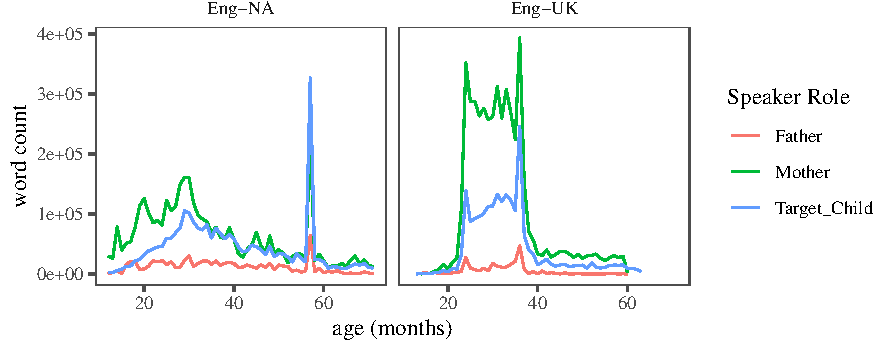
\includegraphics{figs/corpusDensityPlot-1} 

}

\caption{Frequency for all the words in the North America and UK corpora of CHILDES.}\label{fig:corpusDensityPlot}
\end{figure}

\subsubsection{Exclusion Criteria}\label{exclusion-criteria}

First, observations (tokens) that were coded as unintelligible were
excluded (N = 290,119). Second, observations that had missing
information on children's age were excluded (N = 1,042,478). Third,
observations outside the age range of 1 to 6 years were excluded (N =
686,870). This exclusion was because we were interested in the 1 to 6
years old age range and there was not much data outside this age range
either. The mean age is shown with a red vertical line (Mean Age = 3.73,
SD = 2.21). The collection contained the speech of 504 children and
their parents after the exclusions.

\paragraph{Procedure}\label{procedure}

Each token was marked for the utterance type that the token appeared in.
This study grouped utterance types into four main categories:
\enquote{declarative}, \enquote{question}, \enquote{imperative}, and
\enquote{other}. Utterance type categorization followed the convention
used in the
\href{https://talkbank.org/manuals/CHAT.html\#_Toc486414422}{TalkBank
manual}. The utterance types are similar to sentence types (declarative,
interrogative, imperative) with one exception: the category
\enquote{question} consists of interrogatives as well as rising
declaratives (i.e.~declaratives with rising question intonation). In the
transcripts, declaratives are marked with a period, questions with a
question mark, and imperatives with an exclamation mark. It is important
to note that the manual also provides
\href{https://talkbank.org/manuals/CHAT.html\#_Toc486414431}{terminators
for special-type utterances}. Among the special type utterances, this
study included the following in the category \enquote{questions}:
trailing off of a question, question with exclamation, interruption of a
question, and self-interrupted question. The category imperatives also
included \enquote{emphatic imperatives}. The rest of the special type
utterances such as \enquote{interruptions} and \enquote{trailing off}
were included in the category \enquote{other}.\\

\subsubsection{Properties of the CHILDES
Corpora}\label{properties-of-the-childes-corpora}

In this section, I report some results on the distribution of words and
utterances among the speakers in our collection of corpora. The
collection contained 14,159,609 words. Table (\ref{tab:countTable})
shows the total number of \emph{and}'s, \emph{or}'s, and words in the
speech of children, fathers, and mothers. The collection contains 8.80
times more words for mothers compared to fathers and 1.80 more words for
mothers compared to children. Therefore, the collection is more
representative of the mother-child interactions than father-child
interactions. Compared to \emph{or}, the word \emph{and} is 10.80 times
more likely in the speech of mothers, 9.20 times more likely in the
speech of fathers, and 30.30 times more likely in the speech of
children. Overall, \emph{and} is 13.35 times more likely than \emph{or}
in this collection which is close to the rate reported by Morris (2008).
He extracted 5,994 instances of \emph{and} and 465 instances of
\emph{or} and found that overall, \emph{and} was 12.89 times more
frequent than \emph{or} in parent-child interactions.

\begin{table}

\caption{\label{tab:countTable}Number of \textit{and}'s, \textit{or}'s, and the total number of words in the speech of children and their parents in English-North America and English-UK collections after exclusions.}
\centering
\begin{tabular}[t]{l|r|r|r}
\hline
Speaker Role & and & or & total\\
\hline
Father & 15,488 & 1,683 & 967,075\\
\hline
Mother & 153,781 & 14,288 & 8,511,478\\
\hline
Target\_Child & 78,443 & 2,590 & 4,681,056\\
\hline
\end{tabular}
\end{table}

Figure \ref{fig:wordsByAge} shows the number of words spoken by parents
and children at each month of the child's development. The words in the
collection are not distributed uniformly and there is a high
concentration of data between the ages of 20 and 40 months (around 2 to
3 years of age). There is also a high concentration around 60 months (5
years of age). The speech of fathers shows a relatively low word-count
across all ages. Therefore, in our analyses we should be more cautious
in drawing conclusions about the speech of fathers generally, and the
speech of mothers and children after age 5. The distribution of function
words is sensitive to the type of utterance or more broadly the type of
speech act produced by speakers. For example, it is not surprising to
hear a parent say \enquote{go to your room} but a child saying the same
to a parent is unexpected. If a function word commonly occurs in such
speech acts, it is unlikely to be produced by children, even though they
may understand it very well. Therefore, it is important to check the
distribution of speech acts in corpora when studying different function
words. Since it is hard to classify and quantify speech acts
automatically, here I use utterance type as a proxy for speech acts. I
investigate the distribution of declaratives, questions, and imperatives
in this collection of corpora on parent-child interactions. Figure
\ref{fig:totalUtteranceTypePlot} shows the distribution of different
utterance types in the speech of parents and children. Overall, most
utterances are either declaratives or questions, and there are more
declaratives than questions in this collection. While mothers and
fathers show similar proportions of declaratives and questions in their
speech, children produce a lower proportion of questions and higher
proportion of declaratives than their parents.

\begin{figure}[tb]

{\centering 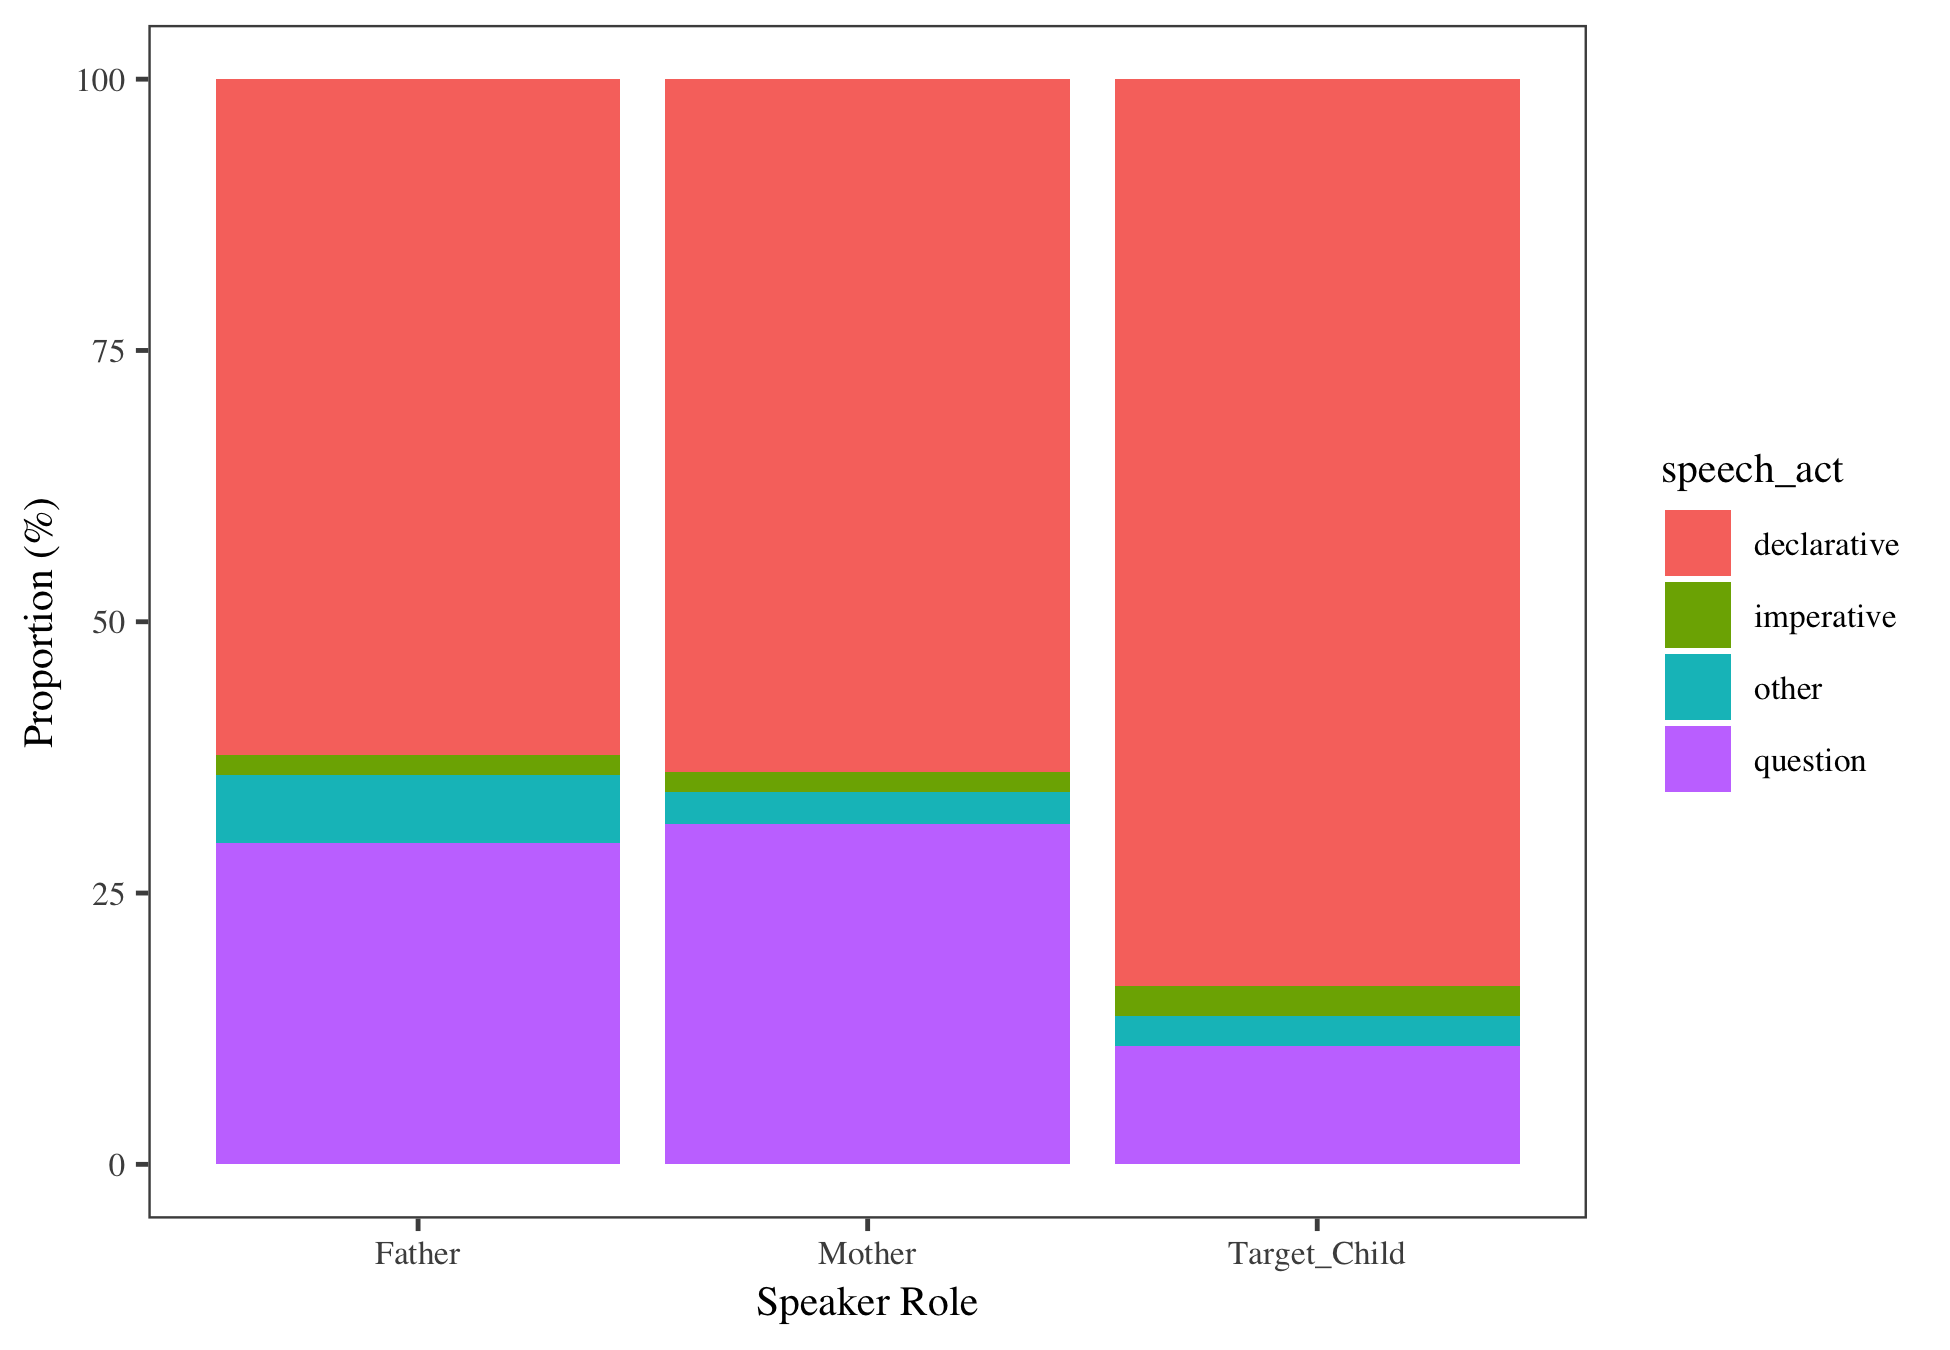
\includegraphics{figs/totalUtteranceTypePlot-1} 

}

\caption{The proportion of declaratives and questions in children's and parents' utterances.}\label{fig:totalUtteranceTypePlot}
\end{figure}

Figure \ref{fig:utteranceTypeByAgePlot} shows the developmental trend of
declaratives and questions between the ages of one and six. Children
start with only producing declaratives and add non-declarative
utterances to their repertoire gradually until they get closer to the
parents' rate around the age six. They also start with very few
questions and increase the number of questions they ask gradually. It is
important to note that the rates of declaratives and questions in
children's speech do not reach the adult rate. These two figures show
that parent-child interactions are asymmetric. Parents ask more
questions and children produce more declaratives. This asymmetry also
interacts with age: the speech of younger children has a higher
proportion of declaratives than older children.

\begin{figure}
\centering
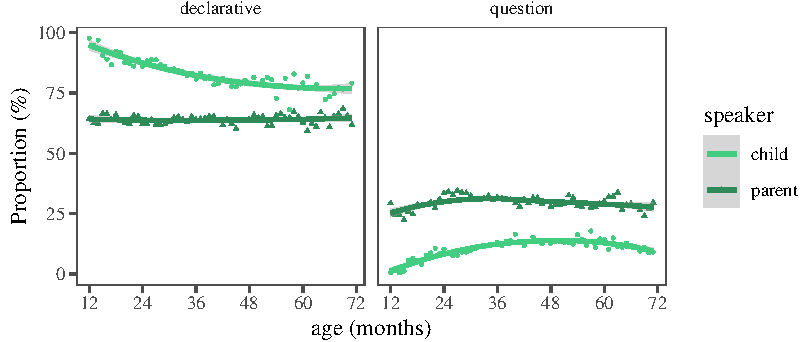
\includegraphics{figs/utteranceTypeByAgePlot-1.pdf}
\caption{\label{fig:utteranceTypeByAgePlot}Proportion of declaratives to
questions in parent-child interactions by age.}
\end{figure}

The frequency of function words such as \emph{and} and \emph{or} may be
affected by such conversational asymmetries if they are more likely to
appear in some utterance types than others. Figure
\ref{fig:CnctPropbySpeechAct} shows the proportion of
\emph{and}\enquote{s and \emph{or}'s that appear in different utterance
types in parents} and children's speech. In parents' speech, \emph{and}
appears more often in declaratives (around 60\% in declaratives and 20\%
in questions). On the other hand, \emph{or} appears more often in
questions than declaratives, although this difference is small in
mothers. In children's speech, both \emph{and} and \emph{or} appear most
often in declaratives. However, children have a higher proportion of
\emph{or} in questions than \emph{and} in questions.

The differences in the distribution of utterance types can affect our
interpretation of the corpus data on function words such as \emph{and}
and \emph{or} in three ways. First, since the collection contains more
declaratives than questions, it may reflect the frequency and diversity
of function words like \emph{and} that appear in declaratives better.
Second, since children produce more declaratives and fewer questions
than parents, we may underestimate children's knowledge of function
words like \emph{or} that are frequent in questions. Third, given that
the percentage of questions in the speech of children increases as they
get older, function words like \emph{or} that are more likely to appear
in questions may appear infrequent in the early stages and more frequent
in the later stages of children's development. In other words, function
words like \emph{or} that are common in questions may show a seeming
delay in production which is possibly due to the development of
questions in children's speech. Therefore, in studying children's
productions of function words, it is important to look at their relative
frequencies in different utterance types as well as the overall trends.
This is the approach I pursue in the next section.

\begin{figure}[tb]

{\centering 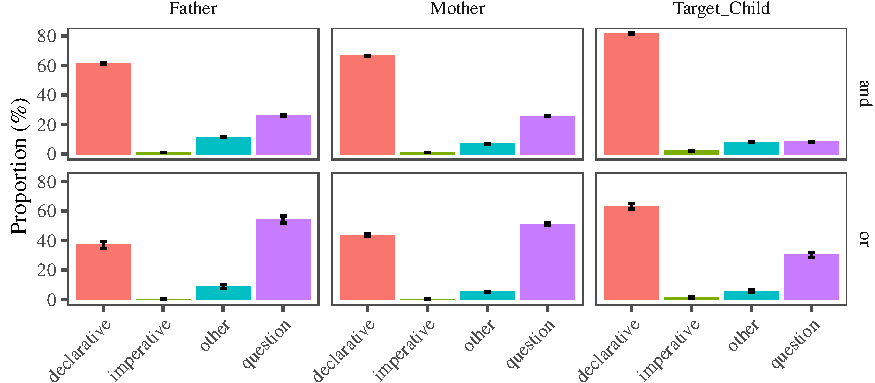
\includegraphics{figs/CnctPropbySpeechAct-1} 

}

\caption{The proportion of \textit{and} and \textit{or} in different utterance types in the speech of parents and children.}\label{fig:CnctPropbySpeechAct}
\end{figure}

\subsubsection{Results}\label{study1results}

First, I consider the overall distribution of \emph{and} and \emph{or}
in the corpora and then look closer at their distributions in different
utterance types. Figure \ref{fig:freqTableBySpeakerPlot} shows the
frequency of \emph{and} and \emph{or} relative to the total number of
words produced by each speaker (i.e.~fathers, mothers, and children).
The y-axes show relative frequency per thousand words. It is also
important to note that the y-axes show different ranges of values for
\emph{and} vs. \emph{or}. This is due to the large difference between
the relative frequencies of these connectives. Overall, \emph{and}
occurs around 15 times per thousand words but \emph{or} only occurs 3
times per 2000 words in the speech of parents and around 1 time every
2000 words in the speech of children. Comparing the relative frequency
of the connectives in parents' and children's speech, we can see that
overall, children and parents produce similar rates of \emph{and} in
their interactions. However, children produce fewer \emph{or}'s than
their parents.

\begin{figure}[tb]

{\centering 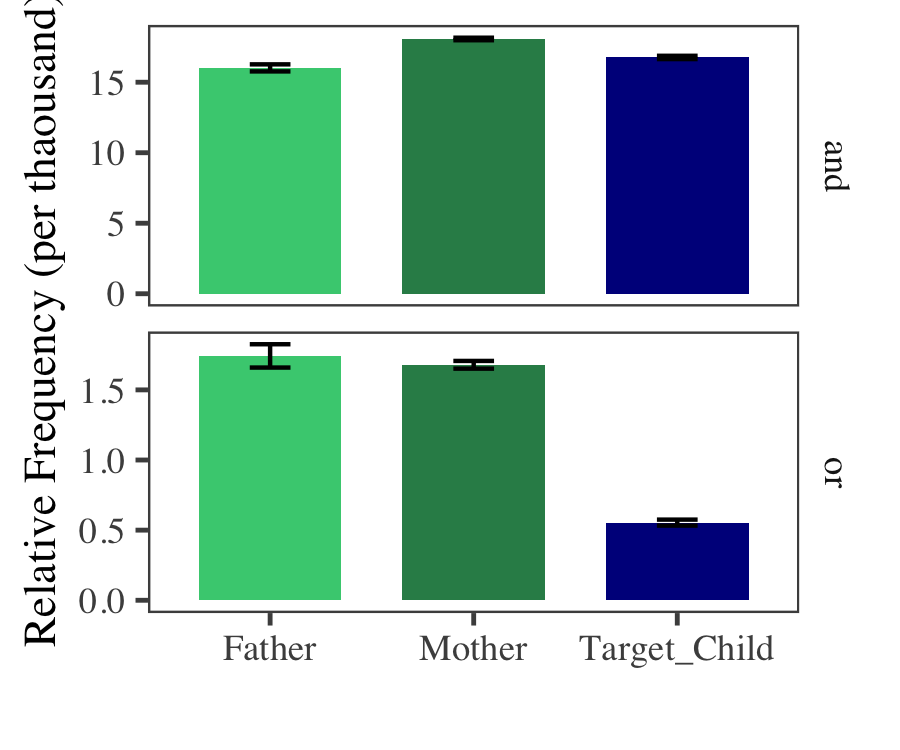
\includegraphics{figs/freqTableBySpeakerPlot-1} 

}

\caption{The relative frequency of \textit{and/or} in the speech of fathers, mothers, and children. 95\% binomial proportion confidence intervals calculated using Agresti-Coull's approximate method.}\label{fig:freqTableBySpeakerPlot}
\end{figure}

Next we look at the relative frequencies of \emph{and} and \emph{or} in
parents and children's speech during the course of children's
development. Figure \ref{fig:agePlot} shows the relative frequencies of
\emph{and} and \emph{or} in parents' and children's speech between 12
and 72 months (1-6 years). Production of \emph{and} in parents' speech
seems to be relatively stable and somewhere between 10 to 20
\emph{and}\enquote{s per thousand words over the course of children's
development. For children, they start producing \emph{and} between 12
and 24 months, and show a sharp increase in their production until they
reach the parent level between 30 to 36 months of age. Children stay
close to the parents} production level between 36 and 72 months,
possibly surpassing them a bit at 60 months -- although as stated in the
previous section, we should be cautious about patterns after 60 months
due to the small amount of data in this period. For \emph{or}, parents
produce between 1 to 2 \emph{or}'s every thousand words and mothers show
a slight increase in their productions between 12 to 36 months. Children
start producing \emph{or} between 18 to 30 months of age. They show a
steady increase in their productions of \emph{or} until they get close
to 1 \emph{or} per thousand words at 48 months (4 years) and stay at
that level until 72 months (6 years).

Children's productions of \emph{and} and \emph{or} show two main
differences. First, the onset of \emph{or} production is later than that
of \emph{and}. Children start producing \emph{and} around 1 to 1.5 years
old while \emph{or} productions start around 6 months later. Second,
children's \emph{and} production shows a steep rise and reaches the
parent level of production at three-years old. For \emph{or}, however,
the rise in children's production level does not reach the parent level
even though it seems to reach a constant level between the ages of 4 and
6 years.

Not reaching the parent level of \emph{or} production does not
necessarily mean that children's understanding of \emph{or} has not
fully developed yet. It can also be due to the nature of parent-child
interactions. For example, since parents ask more questions than
children and \emph{or} appears frequently in questions, parents may have
a higher frequency of \emph{or}. There are two ways of controlling for
this possibility. One is to research children's speech to peers.
Unfortunately such a large database of children's speech to peers is not
currently available for analysis. Alternatively, we can look at the
relative frequencies and developmental trends within utterance types
such as declaratives and questions to see if we spot different
developmental trends. This is what I pursue next. \newline

\begin{figure}[tb]

{\centering 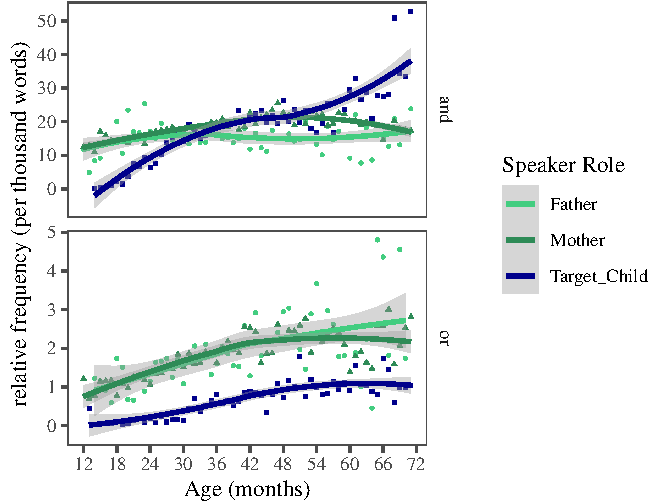
\includegraphics{figs/agePlot-1} 

}

\caption{The monthly relative frequency of \textit{and/or} in parents and children's speech between 12 and 72 months (1-6 years).}\label{fig:agePlot}
\end{figure}

Figure \ref{fig:freqTablebySpeechAct} shows the relative frequency of
\emph{and} and \emph{or} in declaratives, questions, and imperatives.
\emph{And} has the highest relative frequency in declaratives while
\emph{or} has the highest relative frequency in questions. Figure
\ref{fig:ageSpeechActPlot} shows the developmental trends of the
relative frequencies of \emph{and} and \emph{or} in questions and
declaratives. Comparing \emph{and} in declaratives and questions, we see
that the onset of \emph{and} productions are slightly delayed for
questions but in both declaratives and questions, \emph{and} productions
reach the parent level around 36 months (3 years). For \emph{or}, we see
a similar delay in questions compared to declaratives. Children start
producing \emph{or} in declaratives at around 18 months but they start
producing \emph{or} in questions at 24 months. Production of \emph{or}
increases in both declaratives and questions until it seems to reach a
constant rate in declaratives between 48 and 72 months. The relative
frequency of \emph{or} in questions continues to rise until 60 months.
Comparing figures \ref{fig:agePlot} and \ref{fig:ageSpeechActPlot}, we
see that children are closer to the adult rate of production in
declaratives than questions. The large difference between parents and
children's production of \emph{or} in figure \ref{fig:agePlot} may
partly be due to the development of \emph{or} in questions. Overall the
results show that children have a substantial increase in their
productions of \emph{and} and \emph{or} between 1.5 to 4 years of age.
Therefore, it is reasonable to expect that early mappings for the
meaning and usage of these words develop in this age range.

\begin{figure}[tb]

{\centering 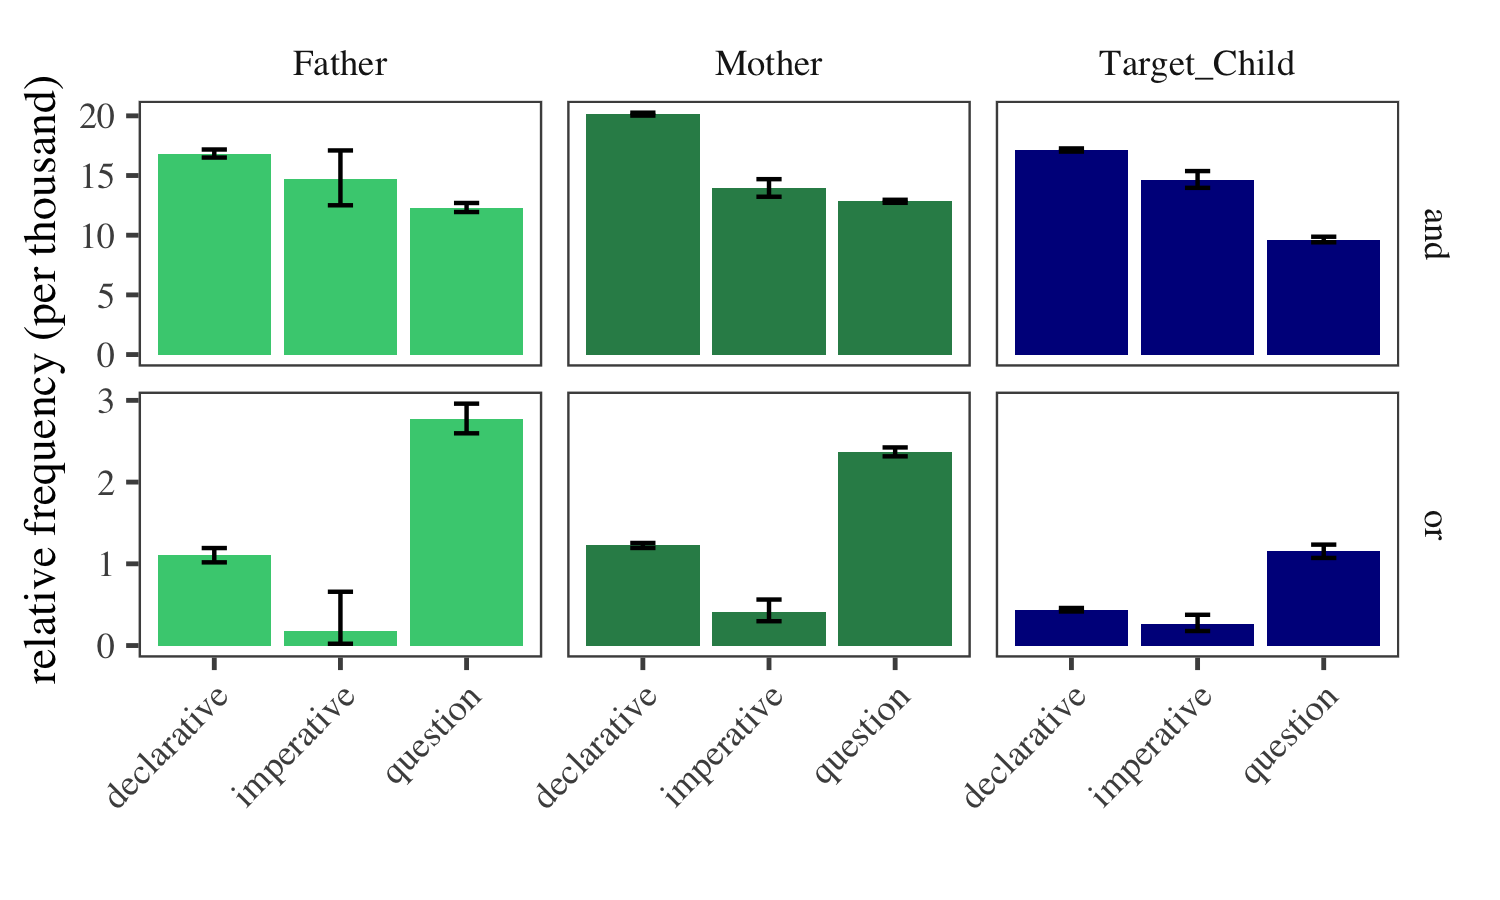
\includegraphics{figs/freqTablebySpeechAct-1} 

}

\caption{Relative frequency of \textit{and/or} in declaratives, imperatives, and interrogatives for parents and children }\label{fig:freqTablebySpeechAct}
\end{figure}

\begin{figure}[tb]

{\centering 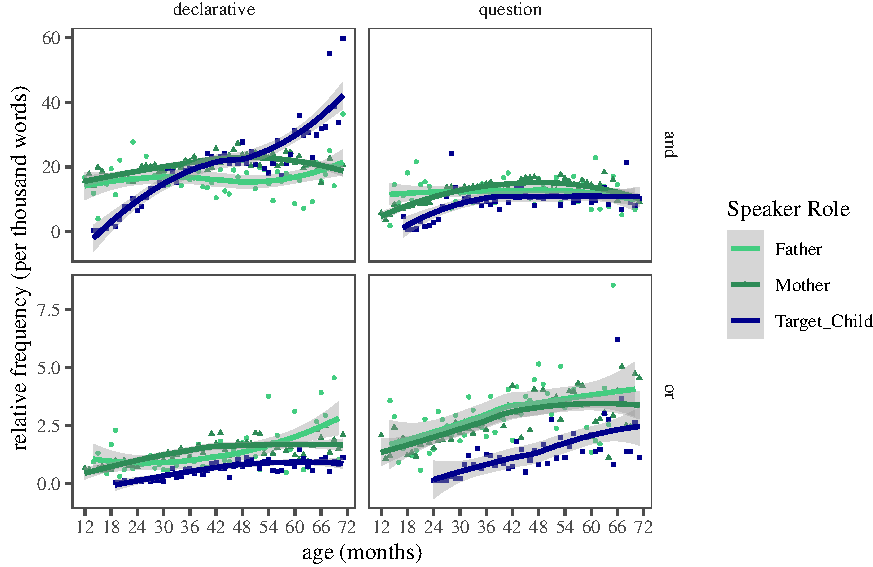
\includegraphics{figs/ageSpeechActPlot-1} 

}

\caption{Relative frequency of \textit{and/or} in declaratives and questions for parents and childern between the child-age of 12 and 72 months (1-6 years).}\label{fig:ageSpeechActPlot}
\end{figure}

\subsubsection{Discussion}\label{study1discussion}

The goal of this study was to explore the frequency of \emph{and} and
\emph{or} in parents and children's speech. The study found three
differences. First, it found a difference between the overall frequency
of \emph{and} and \emph{or} in both parents and children. \emph{And} was
about 10 times more frequent than \emph{or} in the speech of parents and
30 times more likely in the speech of children. Second, the study found
a difference between parents' and children's productions of \emph{or}.
Relative to the total number of words spoken by parents and children
between the ages of 1 and 6 years, both children and parents produce on
average 15 \emph{and}\enquote{s every 1000 words. Therefore, children
match parents} rate of \emph{and} production overall. This is not the
case for \emph{or} as parents produce 3 \emph{or}\enquote{s every 2000
words and children only 1 every 2000 words. Third, the study found a
developmental difference between \emph{and} and \emph{or} as well. The
study found that the onset of production is earlier for \emph{and} than
\emph{or}. In the monthly relative frequencies of \emph{and} and
\emph{or} in the speech of parents and children, the study also found
that children reach the parents} level of production for \emph{and} at
age 3 while \emph{or} does not reach the parents' level even at age 6.

What causes these production differences? The first difference -- that
\emph{and} is far more frequent than \emph{or} -- is not surprising or
limited to child-directed speech. \emph{And} is useful in a large set of
contexts from conjoining elements of a sentence to connecting discourse
elements or even holding the floor and delaying a conversational turn.
In comparison, \emph{or} seems to have a more limited usage. The second
and the third differences -- namely that children produce fewer
\emph{or}\enquote{s than parents, and that they produce \emph{and} and
reach their parents rate earlier than \emph{or} -- could be due to three
factors. First, production of \emph{and} develops and reaches the
parents} rate earlier possibly because it is much more frequent than
\emph{or} in children's input. Previous research suggests that within
the same syntactic category, words with higher frequency in
child-directed speech are acquired earlier (Goodman, Dale, \& Li, 2008).
The conjunction word \emph{and} is at least 10 times more likely than
\emph{or} so earlier acquisition of \emph{and} is consistent with the
effect of frequency on age of acquisition. Second, research on concept
attainment has suggested that the concept of conjunction is easier to
conjure and possibly acquire than the concept of disjunction. In
experiments that participants are asked to detect a pattern in the
classification of cards, participants can detect a conjunctive
classification pattern faster than a disjunctive one (Neisser \& Weene,
1962). Therefore, it is possible that children learn the meaning of
\emph{and} faster and start to produce it earlier but they need more
time to figure out the meaning and usage of \emph{or}.

A third possibility is that the developmental difference between
\emph{and} and \emph{or} is mainly due to the asymmetric nature of
parent-child interactions and the utterance types that each role in this
interaction requires. For example, this study found that parents ask
more questions of children than children do of parents. It also found
that \emph{or} is much more frequent in questions than \emph{and} is.
Therefore, parent-child interaction provides more opportunities for
parents to use \emph{or} than children. In the next study we will
discuss several constructions and communicative functions that are also
more appropriate for the role of parents. For example, \emph{or} is
often used to ask what someone else wants like \enquote{do you want
apple juice or orange juice?} or for asking someone to clarify what they
said such as \enquote{did you mean ball or bowl?}. Both of these
constructions are more likely to be produced by a parent than a child.
\emph{Or} is also used to introduce examples or provide definitions such
as \enquote{an animal, like a rabbit, or a lion, or a sheep}. It is very
unlikely that children would use such constructions to define terms for
parents! Furthermore, such constructions also reveal their own
developmental trends. For example, the study found that children start
by almost entirely producing declaratives and increase their questions
until at age 4 to 6, about 10\% of their utterances are questions.
Therefore, children's ability to produce \emph{or} in a question is
subject to the development of questions themselves. More generally, the
developmental difference between \emph{and} and \emph{or} may also be
due to a difference in the development of other factors that production
of \emph{and} and \emph{or} rely on, such as the development of
constructions with specific communicative functions like unconditionals
(Whether X or Y, discussed in Chapter \ref{sempragLit}). In future
research, it will be important to establish the extent to which each of
these potential causes -- frequency, conceptual complexity, and the
development of other factors such as utterance type or constructions
with specific communicative functions -- contribute to the developmental
differences in the production of conjunction and disjunction.

\section{Study 3: Learning to interpret a
disjunction}\label{study-3-learning-to-interpret-a-disjunction}

In Chapter \ref{sempragLit}, I reviewed the complexities involved in
interpreting a disjunction word such as \emph{or} in English. I showed
that a disjunction can be interpreted as inclusive, exclusive, and even
conjunctive. In addition to these truth-conditional interpretations, a
disjunction is sometimes associated with speaker ignorance/indifference
as well. Given the wide range of interpretations that \emph{or} can
have, how can children learn to interpret it correctly? This is what the
current chapter will address. In doing so, it also provides a potential
solution to the puzzle of learning disjunction mentioned in the
Introduction. To recap the puzzle, previous corpus research as well as
the study in Chapter \ref{corpus}, have shown that the majority of
\emph{or}-examples children hear are exclusive. However, comprehension
studies report that between the ages of three and five, children can
interpret \emph{or} as inclusive disjunction in declarative sentences
(Crain, 2012). The finding of the comprehension studies and the corpus
studies taken together present a learning puzzle: how can children learn
to interpret \emph{or} as inclusive if they mostly hear exclusive
examples? This chapter provides a solution by developing a cue-based
account for children's acquisition of connectives. More generally, the
account proposed in this chapter is helpful for learning words with
multiple interpretations when one interpretation dominates the learner's
input.

Learning from multiple cues is a common approach in language acquisition
(see Monaghan \& Christiansen, 2014, for an overview). In the domain of
function word semantics, Bloom and Wynn (1997) proposed a cue-based
account for the acquisition of number words.

\subsection{Cues to coordinator
meanings}\label{cues-to-coordinator-meanings}

Three important compositional cues can help learners in restricting
their hypotheses to coordinator meanings. First, as pointed out by
Haspelmath (2007), coordination has specific compositional properties.
Coordinators combine two or more units of the same type and return a
larger unit of the same type. The larger unit has the same semantic
relation with the surrounding words as the smaller units would have had
without coordination. These properties separate coordinators from other
function words such as articles, quantifiers, numerals, prepositions,
and auxiliaries which are not used to connect sentences or any two
similar units for that matter. In fact, the special syntactic properties
of coordinators have compelled syntactic theories to consider specific
rules for coordination.

The literature on syntactic bootstrapping suggests that children can use
syntactic properties of the input to limit their word meaning hypotheses
to the relevant domain (Brown, 1957; see Fisher, Gertner, Scott, \&
Yuan, 2010 for a review; Gleitman, 1990). In the current 1073
annotations of conjunction and disjunction, I found that \emph{and} and
\emph{or} connected sentences/clauses 56\% of the time. This pattern is
unexpected for any other class of function words and it is possible that
the syntactic distribution of coordinators cue the learners to the space
of sentential connective meanings.

Second, in the annotation study I found that \emph{and} never occurs
with inconsistent coordinands (e.g. \enquote{clean and dirty}) while
\emph{or} commonly does (e.g. \enquote{clean or dirty}). The
inconsistency of the coordinands can cue the learner to not consider
conjunction as a meaning for the coordinator given that a conjunctive
meaning would too often lead to a contradiction at the utterance level.
On the other hand, choosing disjunction as the meaning avoids this
problem. Third, the large scale study of Chapter \ref{corpus} found that
\emph{or} is more likely to occur in questions than statements while
\emph{and} is more likely in statements. Since questions often contain
more uncertainty while statements are more informative, it is possible
that these environments bias the learner towards selecting hypotheses
that match this general communicative function. Disjunction is less
informative than conjunction and it is possible that the frequent
appearance of \emph{or} in questions cues learners to both its meaning
as a disjunction as well as the ignorance inference commonly associated
with it.

Finally, it is reasonable to assume that not all binary connective
meanings shown in Figure \ref{fig:binaryLogicalConnectivess} are as
likely for mapping. For example, coordinators that communicate
tautologies or contradictions seem to be not good candidates for
informative communication. Similarly, if A coordinated with B simply
asserts the truth of A and says nothing about B, it is unclear why it
would be needed if the language already has the means of simply
asserting A. It is possible that pragmatic principles already bias the
hypothesis space to favor candidates that are communicatively more
efficient.

\begin{figure}[tb]

{\centering 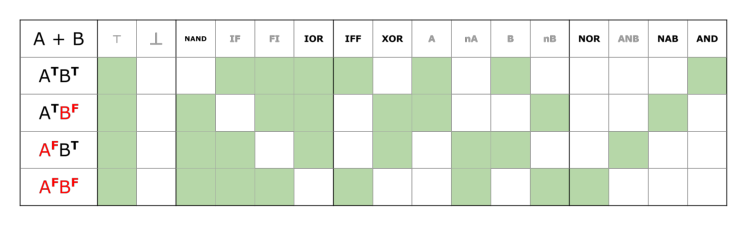
\includegraphics{figs/binaryLogicalConnectivess-1} 

}

\caption{The truth table for the 16 binary logical connectives. The rows represent the set of situations where zero, one, or both propositions are true. The columns represent the 16 possible connectives and their truth conditions. Green cells represent true situations.}\label{fig:binaryLogicalConnectivess}
\end{figure}

Even though these findings are suggestive, they need to be backed up by
further observational and experimental evidence to show that children do
actually use these cues in learning connective meanings. In the next
section, I turn to the more specific issue of learning the correct
interpretation of \emph{and} and \emph{or} from the input data. As in
the case of number words, previous research has provided insight into
how children comprehend a disjunction and what they hear from their
parents. The main question is how children learn what they comprehend
from what they hear. I turn to this issue in the next section.

\subsection{\texorpdfstring{Learning to interpret \emph{and} and
\emph{or}: A cue-based
account}{Learning to interpret and and or: A cue-based account}}\label{myaccount}

Previous comprehension studies as well as the one reported in Chapter
\ref{comprehension} have shown that children as early as age three can
interpret a disjunction as inclusive. However, Morris' (2008) study of
child-directed speech showed that exclusive interpretations are much
more common than other interpretations of disjunction in children's
input. In Figure \ref{fig:interpretation}, I show the results of Chapter
\ref{corpus}\enquote{s annotation study by grouping the disjunction
interpretations into exclusive (EX) and inclusive (IN),
i.e.~non-exclusive categories. These results replicate Morris} (2008)
finding and reinforce a puzzle raised by Crain (2012): How can children
learn the inclusive interpretation of disjunction when the majority of
the examples they hear are exclusive? To answer this question, I draw on
insights from the Gricean approach to semantics and pragmatics discussed
in Chapter \ref{sempragLit}.

\begin{figure}[tb]

{\centering 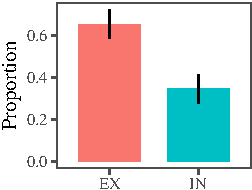
\includegraphics{figs/interpretation-1} 

}

\caption{Proportion of exclusive and inclusive interpretations of disjunction in child-directed speech. Error bars represent bootstrapped 95\% confidence intervals.}\label{fig:interpretation}
\end{figure}

Research in Gricean semantics and pragmatics has shown that the word
\emph{or} is not the only factor relevant to the interpretation of a
disjunction. It is not only the presence of the word \emph{or} that
leads us to interpret a disjunction as inclusive, exclusive, or
conjunctive, but rather the presence of \emph{or} along with several
other factors such as intonation (Pruitt \& Roelofsen, 2013), the
meaning of the disjuncts (Geurts, 2006), and the conversational
principles governing communication (Grice, 1989). The interpretation and
acquisition of the word \emph{or} cannot, therefore, be separated from
all the factors that accompany it and shape its final interpretation.

In the literature on word learning and semantic acquisition,
form-meaning mapping is often construed as mapping an isolated form such
as \emph{gavagai} to an isolated concept such as \enquote{rabbit}. While
this approach may be feasible for content words, it will not work for
function words such as \emph{or}. First, the word \emph{or} cannot be
mapped in isolation from its formal context. As Pruitt and Roelofsen
(2013) showed, the intonation that accompanies a disjunction affects its
interpretation. Therefore, a learner needs to pay attention to the word
\emph{or} as well as the intonation contour that accompanies it. Second,
the word \emph{or} cannot be mapped to its meaning isolated from the
semantics of the disjuncts that accompany it. As Geurts (2006) argued,
the exclusive interpretation is often enforced simply because the
options are incompatible. For example, \enquote{to be or not to be} is
exclusive simply because one cannot both be and not be. In addition,
conversational factors play an important role in the interpretation of
\emph{or} as Grice (1989) argued. In sum, the interpretation and
acquisition of function words such as \emph{or} require the learner to
consider the linguistic and nonlinguistic context of the word and map
the meanings accordingly.

Previous accounts have adopted a model in which a function word such as
\emph{or} is mapped directly to its most likely interpretation:

\emph{or} \(\rightarrow \oplus\)

This model is often used in cross-situational accounts of content words.
Here I argue that the direct mapping of \emph{or} to its interpretation
without consideration of its linguistic context is the primary cause of
the learning puzzle for \emph{or}. Instead, I propose that the word
\emph{or} is mapped to an interpretation in a context-dependent manner,
along with the interpretive cues that accompany it such as intonation
and disjunct semantics:

{[}connective: \emph{or}, Intonation: rise-fall, Disjuncts:
inconsistent{]} \(\rightarrow \oplus\)

{[}connective: \emph{or}, Intonation: rising, Disjuncts: consistent{]}
\(\rightarrow \lor\)

Figure \ref{fig:interpretationByIntonationAndConsistency} shows that the
rate of exclusive interpretations change systematically when the data
are broken down by intonation and consistency. Given a rise-fall
intonation contour, a disjunction is almost always interpreted as
exclusive. Similarly, if the propositions are inconsistent, the
disjunction is most likely interpreted as exclusive. When either of
these two features are absent, a disjunction is more likely to receive
an inclusive interpretation.

\begin{figure}[tb]

{\centering 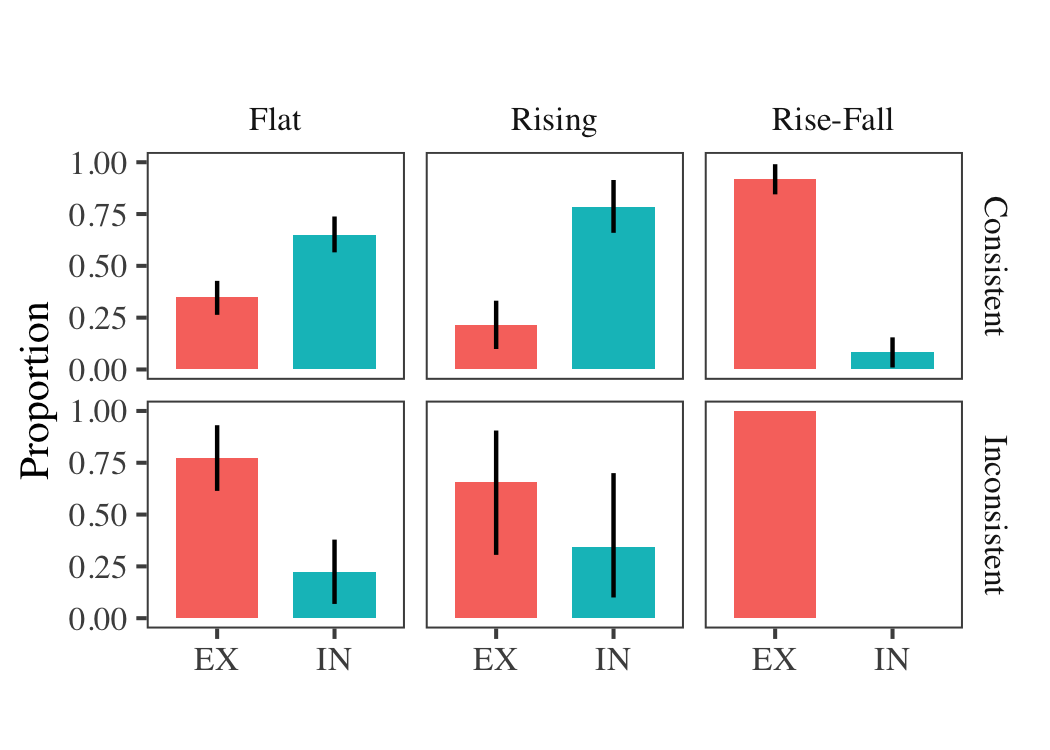
\includegraphics{figs/interpretationByIntonationAndConsistency-1} 

}

\caption{Exclusive and inclusive interpretations broken down by intonation (flat, rise, rise-fall) and consistency. Error bars represent bootstrapped 95\% confidence intervals.}\label{fig:interpretationByIntonationAndConsistency}
\end{figure}

In this account, it is not a single word that gets mapped to an
interpretation but rather a cluster of features. This method has two
advantages. First, it deals with the context dependency of disjunction
interpretation. The learner knows that \emph{or} with some intonation
has to be interpreted differently from one with another. Second, it
allows the learner to pull apart the contribution of \emph{or} from the
interpretive cues that often accompany it. In fact, analysis of all
mapping clusters in which \emph{or} participates and generalization over
them can help the learner extract the semantics of \emph{or} the way it
is intended by Gricean accounts of semantics/pragmatics. For those
skeptical of such an underlying semantics for \emph{or}, there is no
need for further analysis of the mapping clusters. The meaning of
\emph{or} as a single lexical item is distributed among the many
mappings in which it participates. In the next section, I implement this
idea using decision tree learning.

\subsection{Modeling Using Decision Tree Learning}\label{DecisionTrees}

A decision tree is a classification model structured as a hierarchical
tree with nodes, branches, and leaves (Breiman, 2017). The tree starts
with an initial node, called the root, and branches into more nodes
until it reaches the leaves. Each node represents the test on a feature,
each branch represents an outcome of the test, and each leaf represents
a classification label. Using a decision tree, observations can be
classified or labeled based on a set of features.

\emph{I personally wouldn't include this example in a paper,
unnecessary?} For example, we can make a decision tree to predict
whether a food item is a fruit or not based on its color (green or not)
and shape (round or not). An example decision tree is the following: at
the root, the model can ask whether the item is green or not. If yes,
the model creates a leaf and labels the item as \enquote{not fruit}. If
not, the model creates another node and asks if the item is round. If
yes, the item is classified as a \enquote{fruit} and if not it is
classified as \enquote{not fruit}.

Decision trees have several advantages for modeling cue-based accounts
of semantic acquisition. First, decision trees use a set of features to
predict the classification of observations. This is analogous to using
cues to predict the correct interpretation of a word or an utterance.
Second, unlike many other machine learning techniques, decision trees
result in models that are interpretable. Third, the order of decisions
or features used for classification is determined based on information
gain. Features that appear higher (earlier) in the tree are more
informative and helpful for classification. Therefore, decision trees
can help us understand which cues are probably more helpful for the
acquisition and interpretation of a word.

Decision tree learning is the construction of a decision tree from
labeled training data. This section applies decision tree learning to
the annotated data of Chapter \ref{corpus} by constructing random
forests (Breiman, 2001; Ho, 1995). In random forest classification,
multiple decision trees are constructed on subsets of the data, and each
tree predicts a classification. The ultimate outcome is a majority vote
of each trees classification. Since decision trees tend to overfit data,
random forests control for overfitting by building more trees and
averaging their results. \textbf{(Citation)} Next section discusses the
methods used in constrcting the random forests for interpreting
connectives \emph{or}/\emph{and}.

\subsubsection{Methods}\label{methods-1}

The random forest models were constructed using python's Sci-kit Learn
package (Pedregosa et al., 2011). The annotated data had a feature array
and a connective interpretation label for each connective use.
Connective interpretations included exclusive (XOR), inclusive (IOR),
conjunctive (AND), negative inclusive (NOR), and NPQ which states that
only the second proposition is true. The features or cues used included
all other annotation categories: intonation, consistency, syntactic
level, utterance type, and communicative function. All models were
trained with stratified 10-Fold cross-validation to reduce overfitting.
Stratified cross-validation maintains the distribution of the initial
data in the random sampling to build cross validated models. Maintaining
the data distribution ensures a more realistic learning environment for
the forests. Tree success was measured with F1-Score, harmonic average
of precision and recall \textbf{(Citation)}.

First a grid search was run on the hyperparamter space to establish the
number of trees in each forest and the maximum tree depth allowable. The
grid search creates a grid of all combinations of forest size and tree
depth and then trains each forest from this grid on the data. The
forests with the best F1-score and lowest size/depth are reported.
**(Citation*)\textbf{ The default number of trees for the forests was
set to 20, with a max depth of eight and a minimum impurity decrease of
0. Impurity was measured with gini impurity, which states the odds that
a random member of the subset would be mislabled if it were randomly
labeled according to the distribution of labels in the subset.
}(Citation)**

Decision trees were fit with high and low minimum gini decrease values.
High minimum gini decrease results in a tree that does not use any
features for branching. Such a tree represents the baseline or
traditional approach to mapping that directly maps a word to its most
likely interpretation. Low minimum gini decrease allows for a less
conservative tree that uses multiple cues/features to predict the
interpretation of a disjunction. Such a tree represents the cue-based
context-sensitive account of word learning discussed in the previous
section.

\subsubsection{Results}\label{results}

We first present the results of the random forests in the binary
classification task. The models were trained to classify exclusive and
inclusive interpretations of disjunction. For visualization of trees, we
selected the highest performing tree in the forest by testing each tree
and selecting for highest F1 score. While the forests performance is not
identical to the highest performing tree, the best tree gives an
illustrative example of how the tree performs.

Figure \ref{fig:binaryBaseline} shows the best performing decision tree
with high minimum gini decrease. As expected, a learner that does not
use any cues would interpret \emph{or} as exclusive all the time. This
is the baseline model. Figure \ref{fig:binaryCueBased} shows the best
performing decision tree with low minimum gini decrease. The tree has
learned to use intonation and consistency to classify disjunctions as
exclusive or inclusive. As expected, if the intonation is rise-fall or
the disjuncts are inconsistent, the interpretation is exclusive.
Otherwise, the disjunction is classified as inclusive.

\begin{figure}
\centering
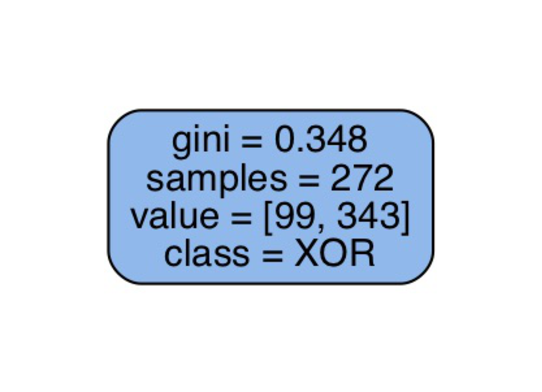
\includegraphics{figs/binaryBaseline-1.pdf}
\caption{\label{fig:binaryBaseline}Baseline tree grown with minimum impurity
decrease of 0.2. The tree always classifies examples of disjunction as
exclusive.}
\end{figure}

\begin{figure}
\centering
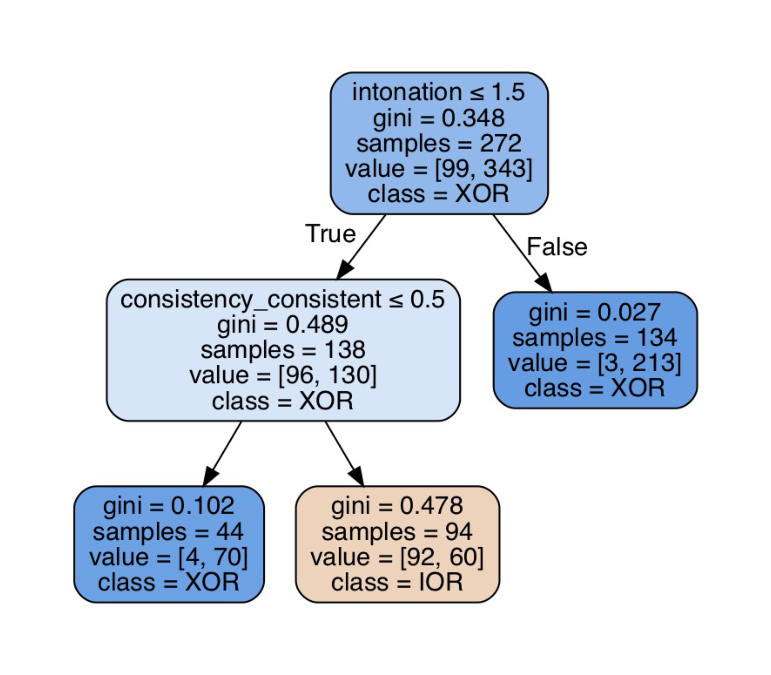
\includegraphics{figs/binaryCueBased-1.pdf}
\caption{\label{fig:binaryCueBased}Cue-based tree grown with minimum
impurity decrease of 0.01. The tree classifies examples of disjunction
with rise-fall intonation as exclusive (intonation \textgreater{} 1.5).
If the intonation is not rise-fall but the disjuncts are inconsistent
(consistency \textless{} 0.5), then the disjunction is still classified
as exclusive. However, if neither of these two hold, the disjunction is
classified as inclusive.}
\end{figure}

Figure \ref{fig:XorBinary} shows the average F1 scores of the baseline
and cue-based models in classifying exclusive examples. The models
perform relatively well and similar to each other, but the cue-based
model performs slightly better. The real difference between the baseline
model and the cue-based model is in their performance on inclusive
examples. Figure \ref{fig:IorBinary} shows the F1 score of the forests
as a function of the training size in classifying inclusive examples. As
expected, the baseline model performs very poorly while the cue-based
model does a relatively good job and improves with more examples.

\begin{figure}
\centering
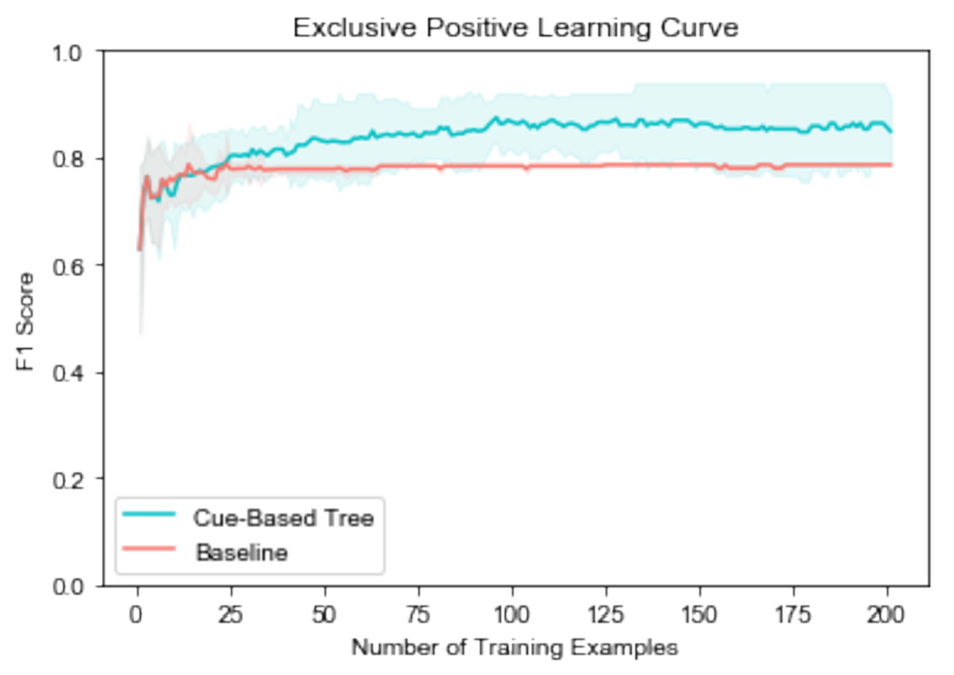
\includegraphics{figs/XorBinary-1.pdf}
\caption{\label{fig:XorBinary}The average F1 score for class XOR (exclusive)
as a function of the number of training examples in the baseline and
cue-based models. The colored shades show the 95\% confidence
intervals.}
\end{figure}

\begin{figure}
\centering
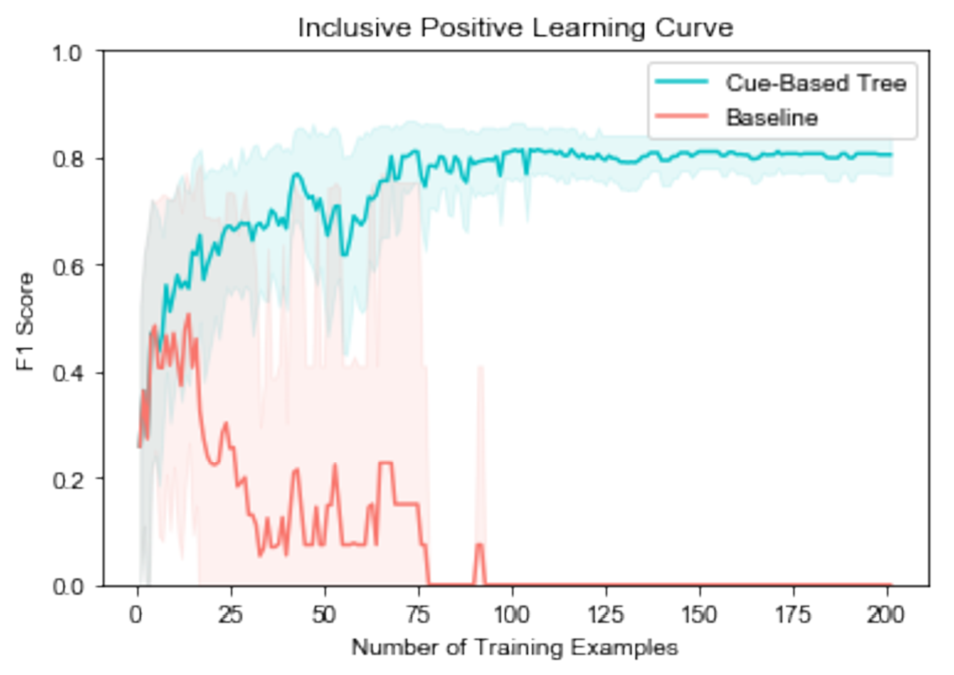
\includegraphics{figs/IorBinary-1.pdf}
\caption{\label{fig:IorBinary}The average F1 score for class IOR (inclusive)
as a function of the number of training examples in the baseline and
cue-based models. The colored shades show the 95\% confidence
intervals.}
\end{figure}

Next, we use decision tree learning in a ternary classification task.
The model uses features to interpret a coordination with \emph{and} and
\emph{or} as inclusive (IOR), exclusive (XOR), or conjunctive (AND).
Figure \ref{fig:ternaryBaseline} shows the baseline decision tree with
high minimum gini decrease, which only uses the presence of the words
\emph{or}/\emph{and} to interpret conjunction and disjunction. As
expected, the tree interprets a coordination with \emph{and} as a
conjunction and one with \emph{or} as exclusive disjunction. Figure
\ref{fig:ternaryCueBased} shows the cue-based decision tree with low
minimum gini decrease. In addition to the presence of \emph{and} and
\emph{or}, the tree uses intonation, consistency, communicative
function, and utterance type to distinguish exclusive, inclusive, and
conjunctive uses of disjunction. In short, a disjunction that is
rise-fall, inconsistent, or has a conditional communicative function is
classified as exclusive. Otherwise the disjunction is classified as
inclusive. The tree also finds conjunctive interpretations of
disjunction more likely in declarative sentences than interrogatives.

\begin{figure}
\centering
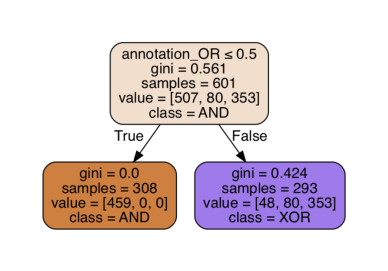
\includegraphics{figs/ternaryBaseline-1.pdf}
\caption{\label{fig:ternaryBaseline}The baseline tree grown on conjunctions
and disjunctions with minimum impurity decrease of 0.2. The tree uses
the words \textit{and/or} and classifies them as conjunction and
exclusive disjunction respectively.}
\end{figure}

\begin{figure}
\centering
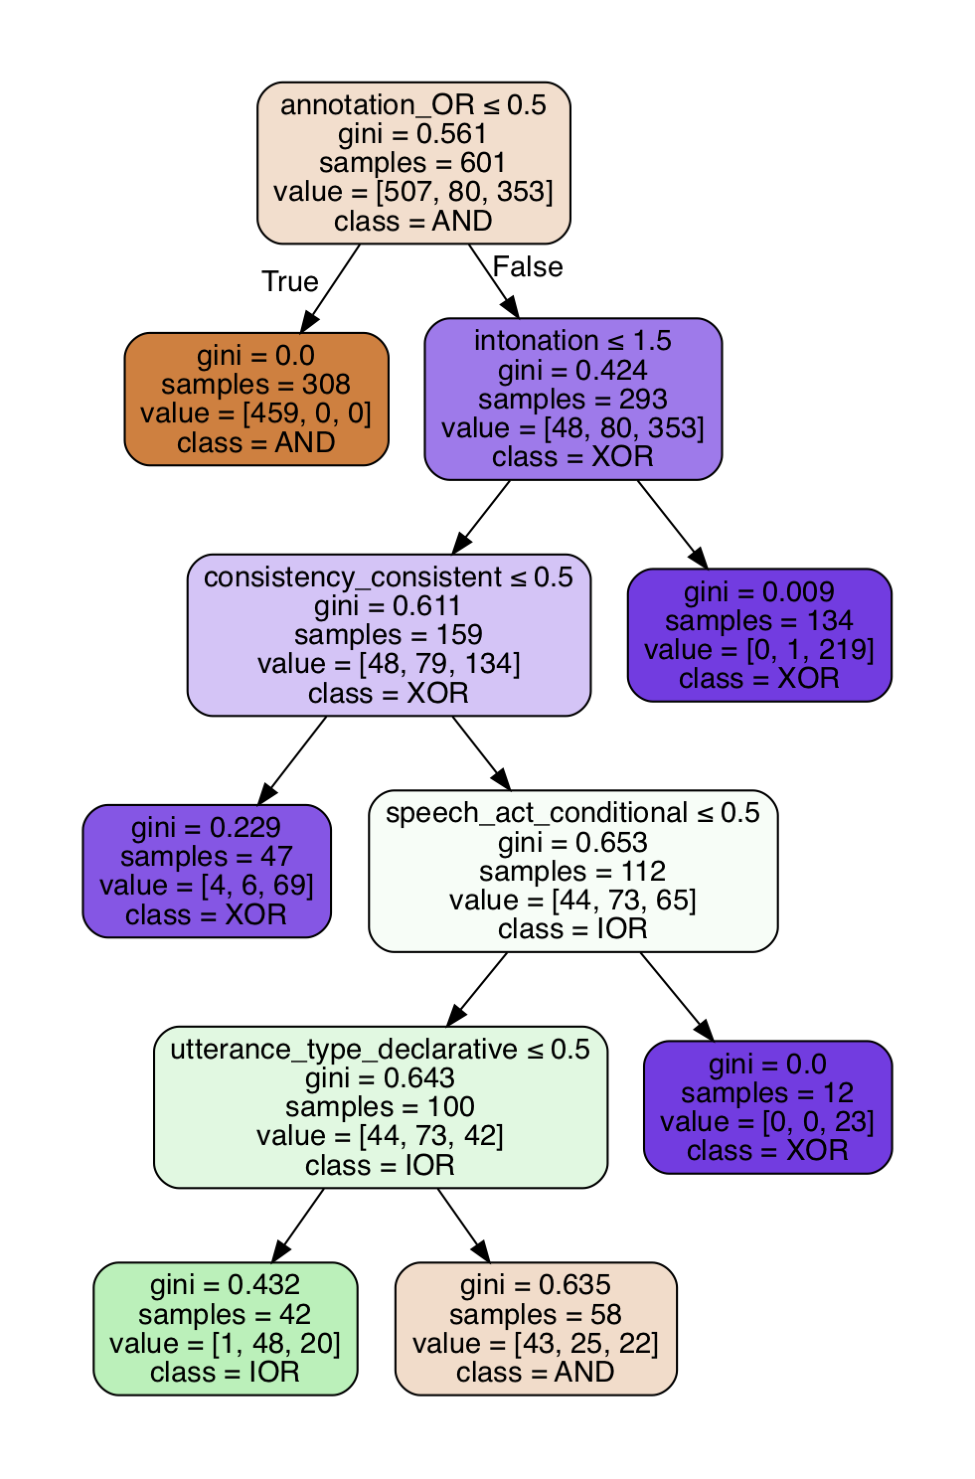
\includegraphics{figs/ternaryCueBased-1.pdf}
\caption{\label{fig:ternaryCueBased}The cue-based tree grown on conjunctions
and disjunctions with minimum impurity decrease of 0.01. After using the
words \textit{and/or}, the tree uses intonation, consistency, and the
conditional communicative function to classify a large number of
exclusive cases. Then it uses utterance type (interrogative) to label
inclusive cases.}
\end{figure}

Figure \ref{fig:ANDintermediate} shows the average F1 score of the
conjunctive interpretations (AND) for the baseline and the cue-based
models. Since the vast majority of the conjunctive interpretations are
predicted by the presence of the word \emph{and}, the baseline and
cue-based models show similar performances. Setting aside conjunction
examples, Figure \ref{fig:ANDintermediateDis} shows the average F1 score
of the AND interpretation of disjunction only. Here we see that the
cue-based model performs better than the default model in guessing
conjunctive interpretations of disjunction. The informal analysis of the
trees suggest that the model does this by using the \enquote{speech act}
cue. Figure \ref{fig:XORintermediate} shows the average F1-score of the
exclusive interpretations (XOR) for the baseline and the cue-based
models. The cue-based model does slightly better than the baseline
model. As before, the most important improvement comes in identifying
inclusive examples. Figure \ref{fig:IORintermediate} shows the average
F1-score of the inclusive interpretations (IOR) for both baseline and
cue-based models. The baseline model performs very poorly while the
cue-based model is capable of classifying inclusive examples as well.

\begin{figure}
\centering
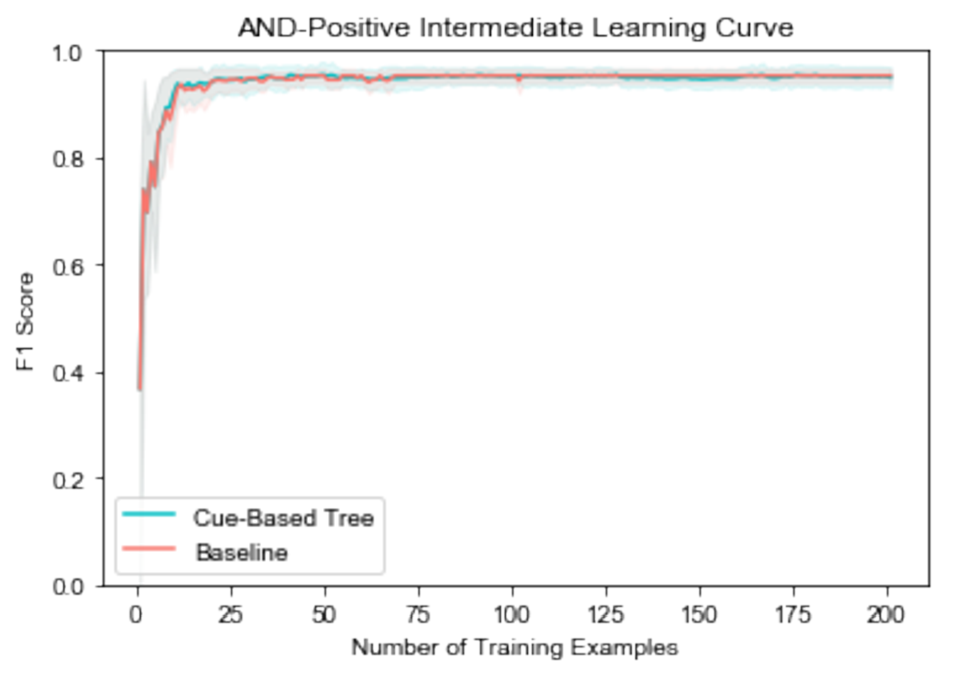
\includegraphics{figs/ANDintermediate-1.pdf}
\caption{\label{fig:ANDintermediate}The average F1 score for class AND as a
function of the number of training examples in the baseline and
cue-based models. The colored shades show the 95\% confidence
intervals.}
\end{figure}

\begin{figure}
\centering
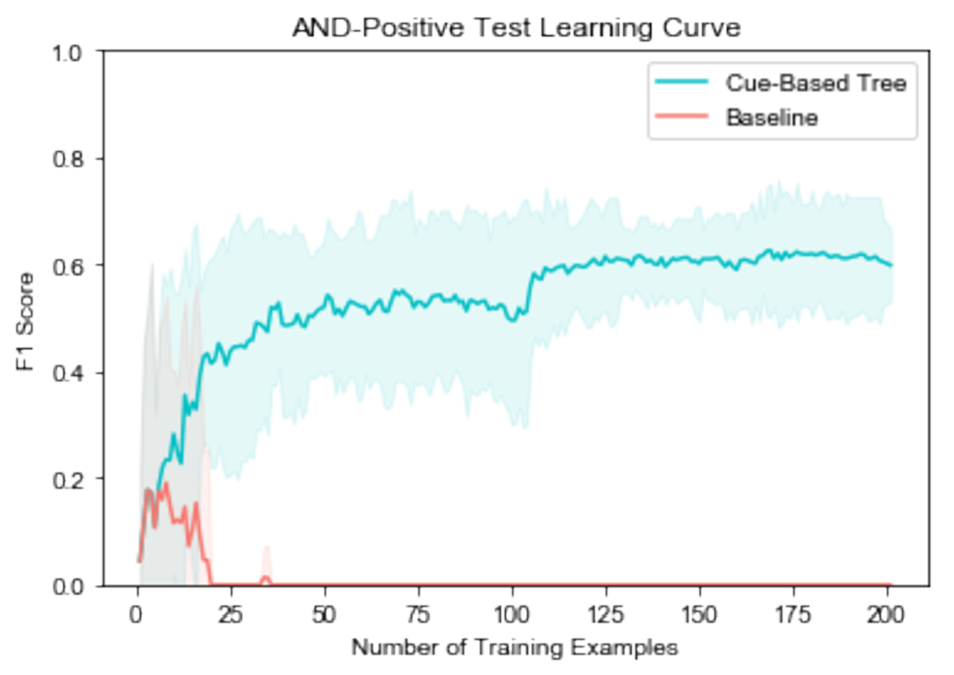
\includegraphics{figs/ANDintermediateDis-1.pdf}
\caption{\label{fig:ANDintermediateDis}The average F1 score for class AND of
disjunction examles as a function of the number of training examples in
the baseline and cue-based models. The colored shades show the 95\%
confidence intervals.}
\end{figure}

\begin{figure}
\centering
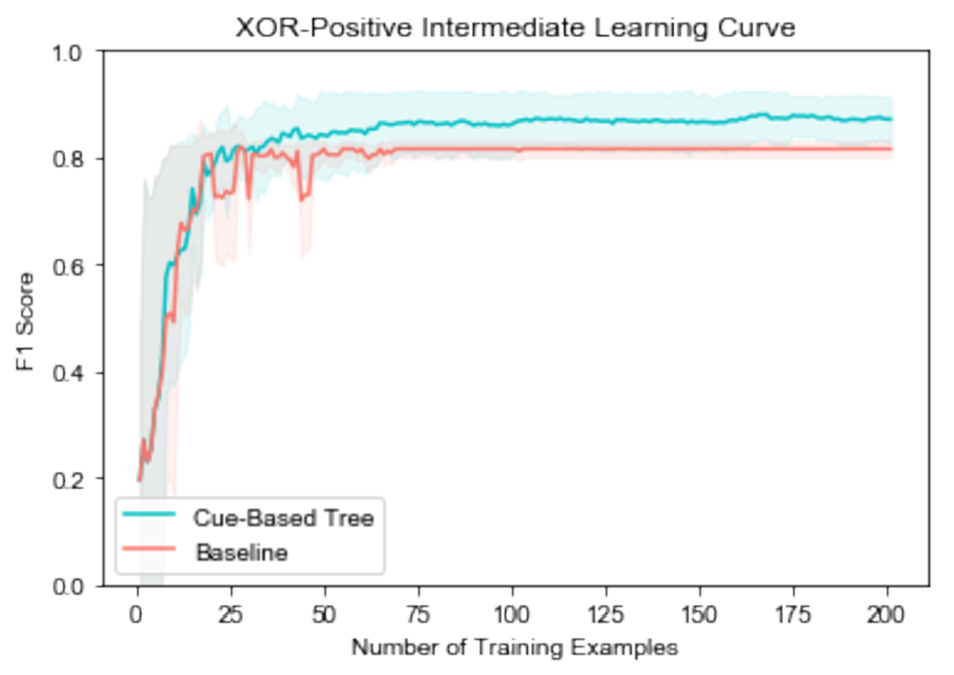
\includegraphics{figs/XORintermediate-1.pdf}
\caption{\label{fig:XORintermediate}The average F1 score for class XOR as a
function of the number of training examples in the baseline and
cue-based models. The colored shades show the 95\% confidence
intervals.}
\end{figure}

\begin{figure}
\centering
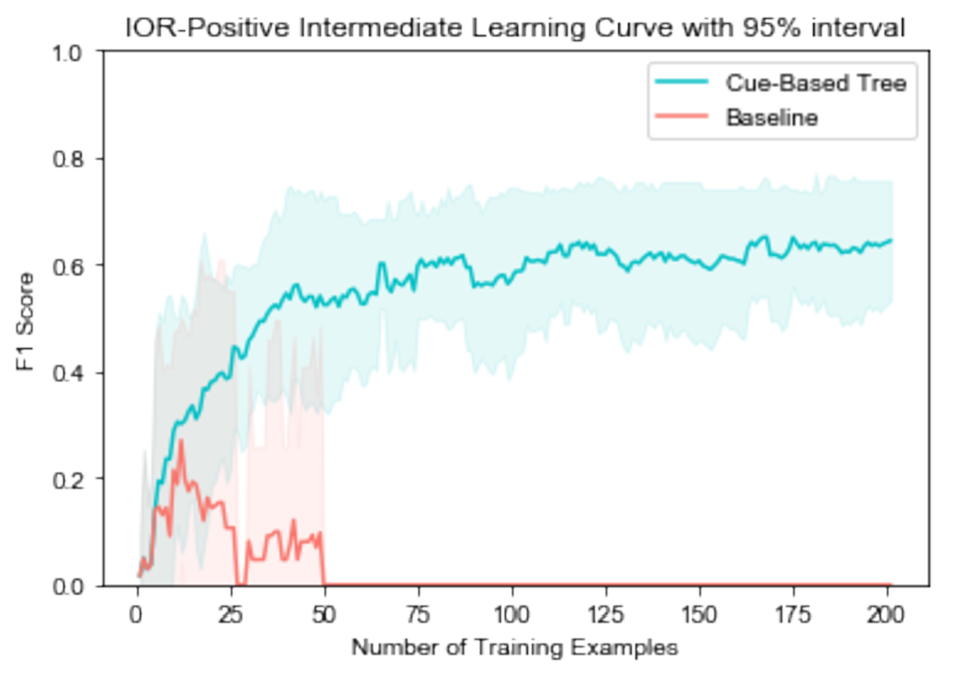
\includegraphics{figs/IORintermediate-1.pdf}
\caption{\label{fig:IORintermediate}The average F1 score for class IOR as a
function of the number of training examples in the baseline and
cue-based models. The colored shades show the 95\% confidence
intervals.}
\end{figure}

Finally, welook at decision trees trained on the annotation data to
predict all the interpretation classes for disjunction: AND, XOR, IOR,
NOR, and NPQ. Figure \ref{fig:wholeBaseline} shows the baseline model
that only uses the words \emph{and} and \emph{or} to classify. As
expected, \emph{and} receives a conjunctive interpretation (AND) and
\emph{or} receives an exclusive interpretation (XOR). Figure
\ref{fig:wholeCueBased} shows the best example tree of the cue-based
model. The leaves of the tree show that it recognizes exclusive,
inclusive, conjunctive, and even negative inclusive (NOR)
interpretations of disjunction. How does the tree achieve that? Like the
baseline model, the tree first asks about the connective used:
\emph{and} vs. \emph{or}. Then like the previous models, it asks about
intonation and consistency. If the intonation is rise-fall, or the
disjuncts are inconsistent, the interpretation is exclusive. Then it
asks whether the sentence is an interrogative or a declarative. If
interrogative, it guesses an inclusive interpretation. This basically
covers questions with a rising intonation. Then the tree picks
declarative examples that have conditional speech act (e.g.
\enquote{give me the toy or you're grounded}) and labels them as
exclusive. Finally, if negation is present in the sentence, the tree
labels the disjunction as NOR.

\begin{figure}
\centering
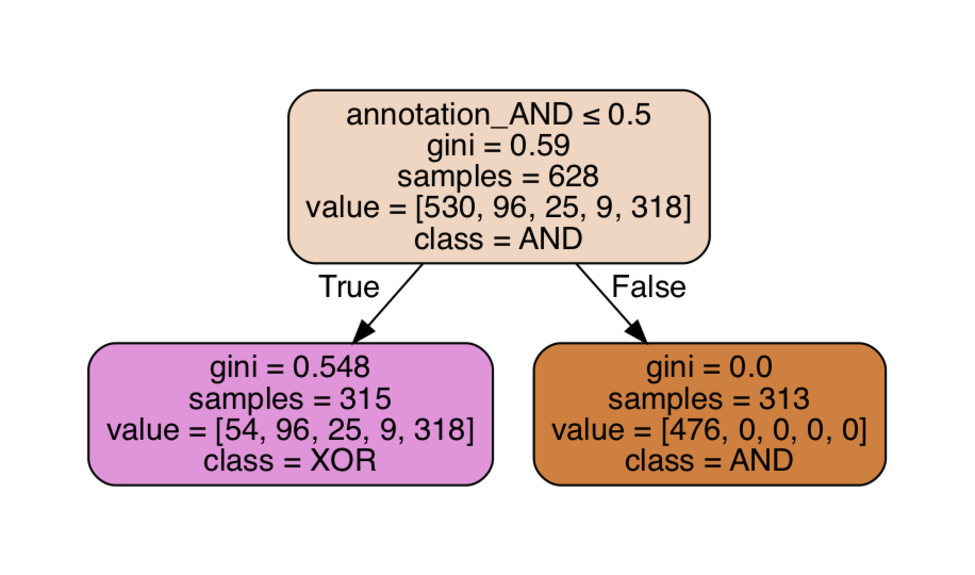
\includegraphics{figs/wholeBaseline-1.pdf}
\caption{\label{fig:wholeBaseline}The baseline tree grown on conjunctions
and disjunctions with minimum impurity decrease of 0.2. The tree uses
the words \textit{and/or} and classifies them as conjunction and
exclusive disjunction.}
\end{figure}

\begin{figure}
\centering
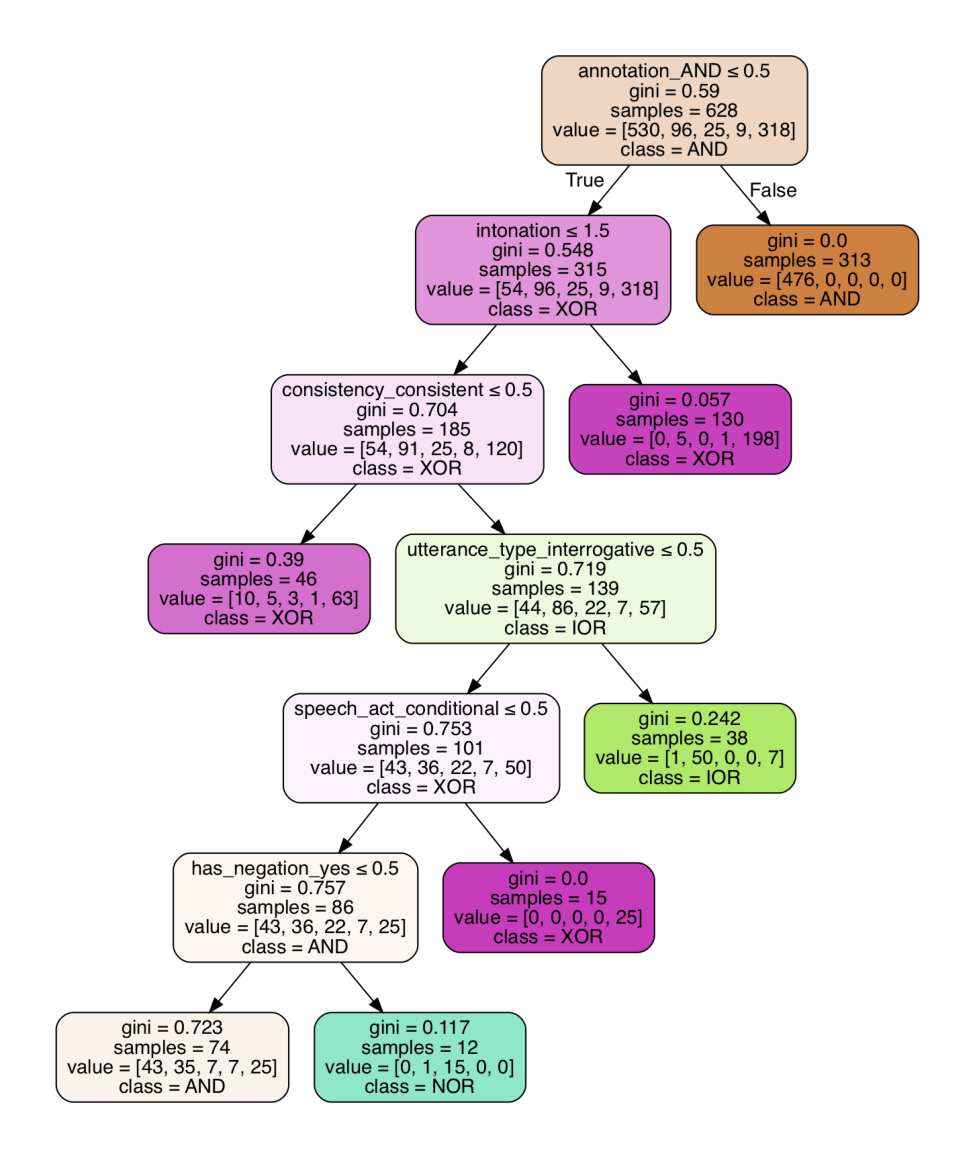
\includegraphics{figs/wholeCueBased-1.pdf}
\caption{\label{fig:wholeCueBased}The cue-based tree grown on conjunctions
and disjunctions with minimum impurity decrease of 0.01. After using the
words \textit{and/or}, the tree uses intonation and consistency to
classify a large number of exclusive cases. Then it uses utterance type
(interrogative) to label many inclusive cases, as well as the
communicative function (conditional) to catch more exclusive examples.
Finally, it asks whether the sentence has negation or not. If so, it
classifies the negative inlusive examples as NOR.}
\end{figure}

Figures \ref{fig:ANDWhole}, \ref{fig:XORWhole}, and \ref{fig:IORWhole}
show the average F1-scores for the conjunctive (AND), exclusive (XOR),
and inclusive (IOR) interpretations as a function of training size. The
results are similar to what wereported before with the ternary
classification. While the cue-based model generally performs better than
the baseline model, it shows substantial improvement in classifying
inclusive cases.

\begin{figure}
\centering
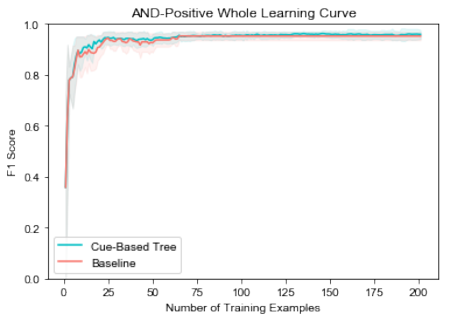
\includegraphics{figs/ANDWhole-1.pdf}
\caption{\label{fig:ANDWhole}The average F1 score for class AND as a
function of the number of training examples in the baseline and
cue-based models. The colored shades show the 95\% confidence
intervals.}
\end{figure}

\begin{figure}
\centering
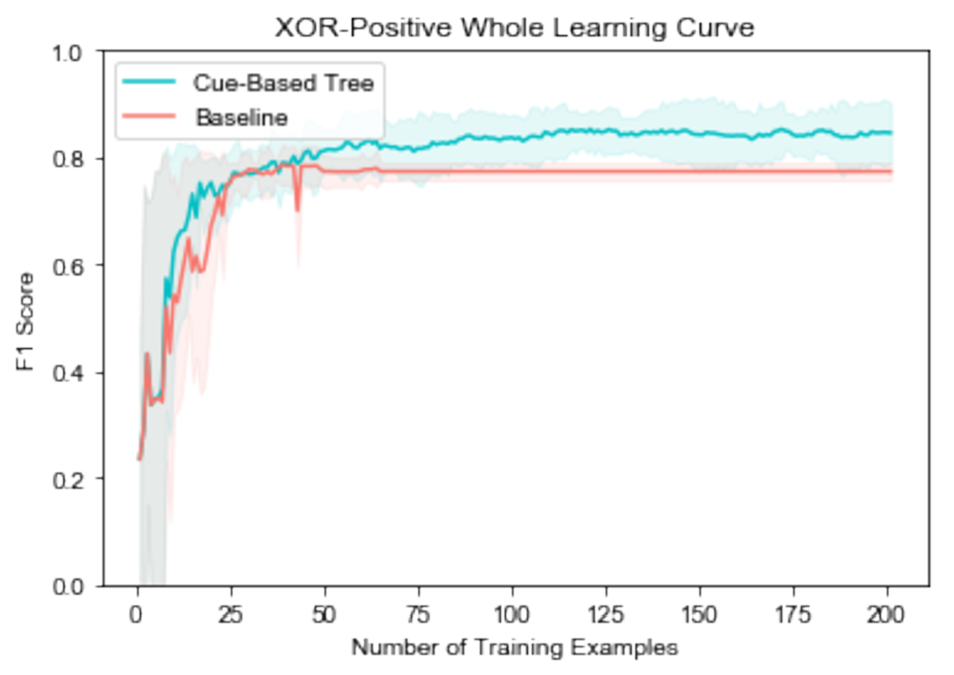
\includegraphics{figs/XORWhole-1.pdf}
\caption{\label{fig:XORWhole}The average F1 score for class XOR as a
function of the number of training examples in the baseline and
cue-based models. The colored shades show the 95\% confidence
intervals.}
\end{figure}

\begin{figure}
\centering
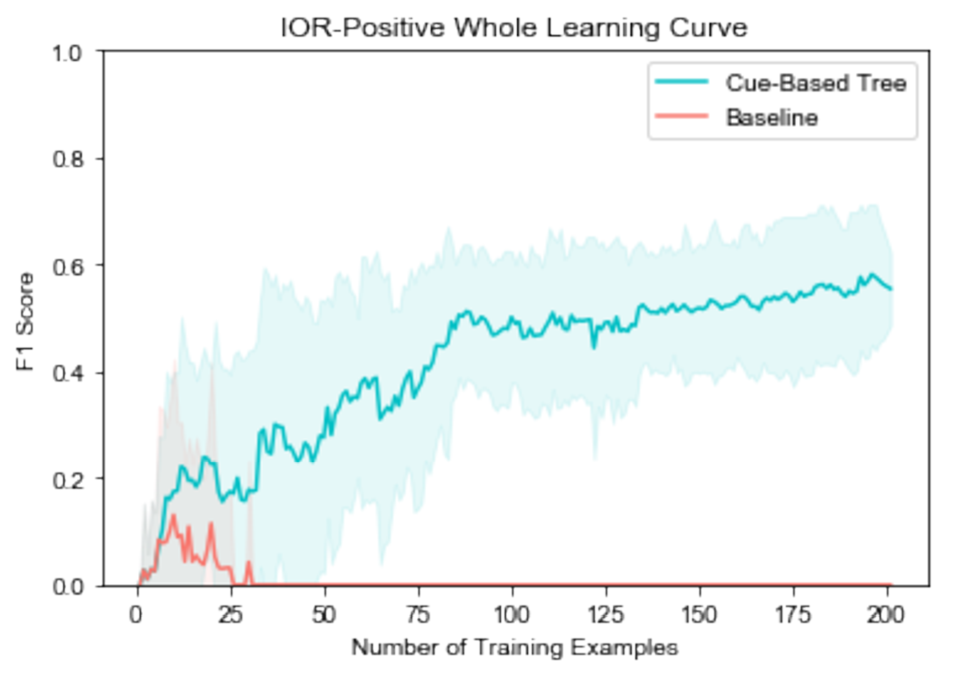
\includegraphics{figs/IORWhole-1.pdf}
\caption{\label{fig:IORWhole}The average F1 score for class IOR as a
function of the number of training examples in the baseline and
cue-based models. The colored shades show the 95\% confidence
intervals.}
\end{figure}

Figure \ref{fig:NORWhole} shows the average F1-score for the negative
inclusive interpretation as a function of training size. Compared to the
baseline model, the cue-based model shows a substantially better
performance in classifying negative sentences. The success of the model
in classifying negative inclusive examples (NOR) suggests that the
cue-based model offers a promising approach for capturing the scope
relation of operators such as negation and disjunction. Here, the model
learns that when negation and disjunction are present, the sentence
receives a negative inclusive (NOR) interpretation. In other words, the
model has learned the narrow-scope interpretation of negation and
disjunction from the input data. In a language where negation and
disjunction receive an XOR interpretation (not A or not B), the
cue-based model can learn the wide-scope interpretation of disjunction.

\begin{figure}
\centering
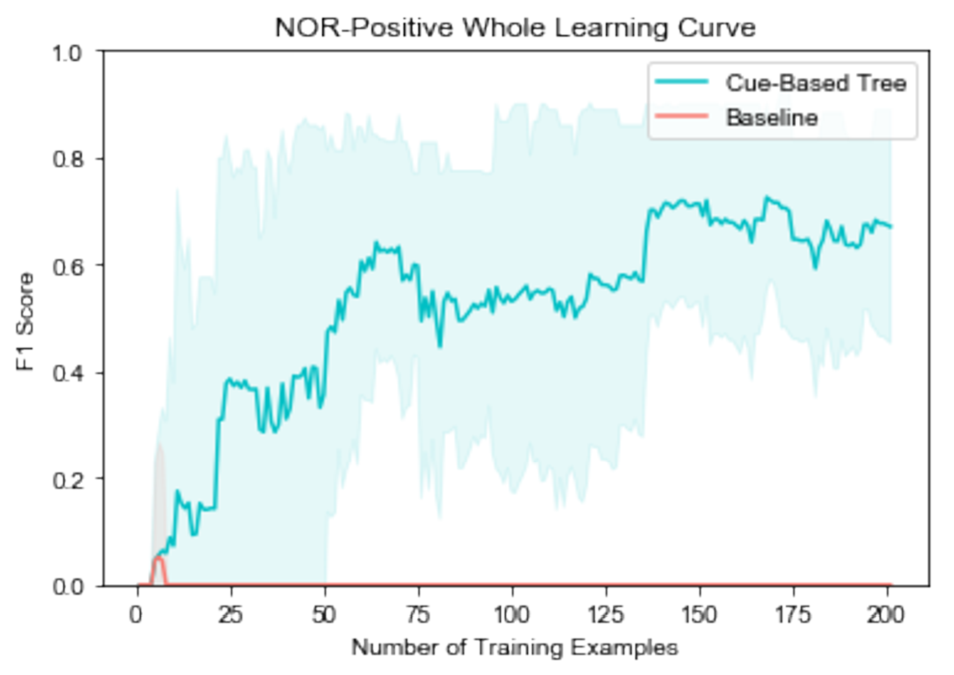
\includegraphics{figs/NORWhole-1.pdf}
\caption{\label{fig:NORWhole}The average F1 score for class NOR as a
function of the number of training examples in the baseline and
cue-based models. The colored shades show the 95\% confidence
intervals.}
\end{figure}

Finally, Figure \ref{fig:NPQWhole} shows the average F1 score for the
class NPQ. This interpretation suggested that the first disjunct is
false but the second true. It was seen in examples of repair most often
and the most likely cue to it was also the communicative function or
speech act of repair. The results show that even though there were
improvements in the cue-based model, they were not stable as shown by
the large confidence intervals. It is possible that with larger training
samples, the cue-based model can reliably classify the NPQ
interpretations as well.

\begin{figure}
\centering
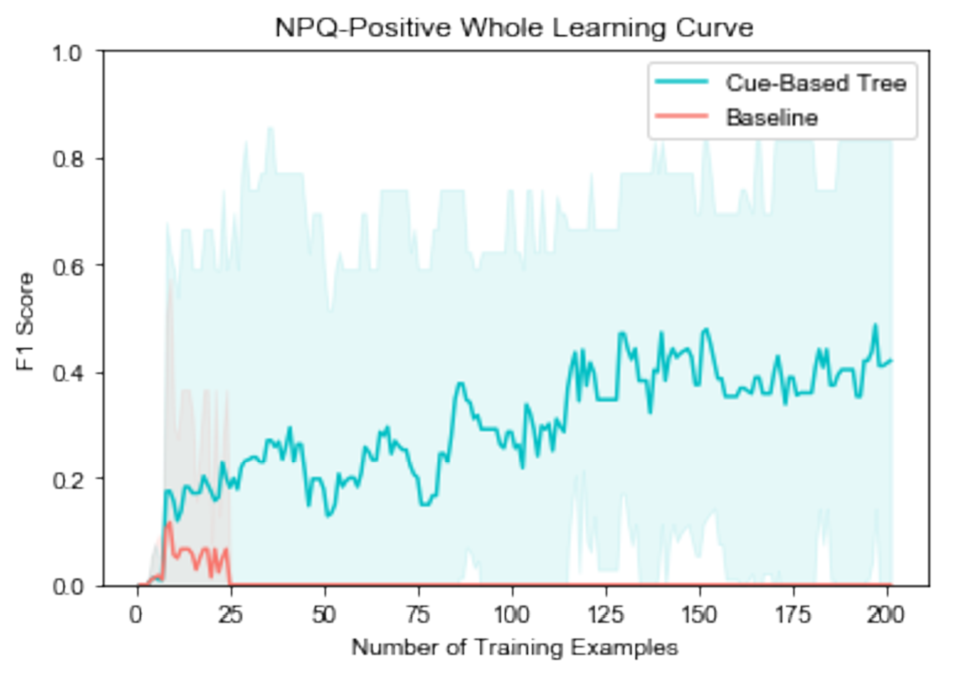
\includegraphics{figs/NPQWhole-1.pdf}
\caption{\label{fig:NPQWhole}The average F1 score for class NPQ as a
function of the number of training examples in the baseline and
cue-based models. The colored shades show the 95\% confidence
intervals.}
\end{figure}

\subsection{Discussion}\label{discussion}

In this chapter, we discussed two accounts for the acquisition of
function words. The first account was a baseline (context-independent)
account that is used in vanilla cross-situational word learning: words
are isolated and directly mapped to their most frequent meanings. The
second account is what I called the cue-based context-dependent mapping
in which words are mapped to meanings conditional on a set of present
cues in the context. I argued that the puzzle of learning disjunction
arises because in the baseline account, forms are mapped directly to
meanings without considering the context of use. Under this account, the
input statistics supports an exclusive interpretation for \emph{or}.
However, comprehension studies show that children can interpret
\emph{or} as inclusive. I showed that the cue-based account resolves
this problem by allowing \emph{or} to be mapped to its interpretation
according to the set of contextual cues that disambiguate it. The
results of computational experiments with decision tree learning on data
from child-directed speech suggested that such an approach can
successfully learn to classify a disjunction is inclusive or exclusive.
More broadly, cue-based context-dependent mapping is useful for the
acquisition of ambiguous words and interpretations that are consistent
but relatively infrequent in child-directed speech.

\section{Conclusion}\label{conclusion}

\newpage

\section{References}\label{references}

\section{Appendix}\label{appendix}

\subsection{Inter-annotator agreement}\label{inter-annotator-agreement}

\setlength{\parindent}{-0.5in} \setlength{\leftskip}{0.5in}

\hypertarget{refs}{}
\hypertarget{ref-bloom1997linguistic}{}
Bloom, P., \& Wynn, K. (1997). Linguistic cues in the acquisition of
number words. \emph{Journal of Child Language}, \emph{24}(3), 511--533.

\hypertarget{ref-breiman2001random}{}
Breiman, L. (2001). Random forests. \emph{Machine Learning},
\emph{45}(1), 5--32.

\hypertarget{ref-breiman2017classification}{}
Breiman, L. (2017). \emph{Classification and regression trees}. London:
Routledge.

\hypertarget{ref-brown1957linguistic}{}
Brown, R. (1957). Linguistic determinism and the part of speech.
\emph{The Journal of Abnormal and Social Psychology}, \emph{55}(1), 1.

\hypertarget{ref-crain2012emergence}{}
Crain, S. (2012). \emph{The emergence of meaning}. Cambridge: Cambridge
University Press.

\hypertarget{ref-fisher2010syntactic}{}
Fisher, C., Gertner, Y., Scott, R. M., \& Yuan, S. (2010). Syntactic
bootstrapping. \emph{Wiley Interdisciplinary Reviews: Cognitive
Science}, \emph{1}(2), 143--149.

\hypertarget{ref-geurts2006exclusive}{}
Geurts, B. (2006). Exclusive disjunction without implicatures.
\emph{Ms., University of Nijmegen}.

\hypertarget{ref-gleitman1990structural}{}
Gleitman, L. (1990). The structural sources of verb meanings.
\emph{Language Acquisition}, \emph{1}(1), 3--55.

\hypertarget{ref-goodman2008does}{}
Goodman, J. C., Dale, P. S., \& Li, P. (2008). Does frequency count?
Parental input and the acquisition of vocabulary. \emph{Journal of Child
Language}, \emph{35}(3), 515--531.

\hypertarget{ref-grice1989studies}{}
Grice, H. P. (1989). \emph{Studies in the way of words}. Cambridge, MA:
Harvard University Press.

\hypertarget{ref-haspelmath2007}{}
Haspelmath, M. (2007). Coordination. In T. Shopen (Ed.), \emph{Language
typology and linguistic description,} Cambridge: Cambridge University
Press.

\hypertarget{ref-ho1995random}{}
Ho, T. K. (1995). Random decision forests. In \emph{Proceedings of the
third international conference on document analysis and recognition}
(Vol. 1, pp. 278--282). Washington, DC, USA: IEEE Computer Society.

\hypertarget{ref-macwhinney2000childes}{}
MacWhinney, B. (2000). \emph{The CHILDES project: The database} (Vol.
2). Mahwah, NJ: Erlbaum.

\hypertarget{ref-monaghan2014multiple}{}
Monaghan, P., \& Christiansen, M. (2014). Multiple cues in language
acquisition. In P. Brooks \& V. Kempe (Eds.), \emph{Encyclopedia of
language development} (pp. 389--392). Thousand Oaks, CA: Sage
Publications.

\hypertarget{ref-morris2008logically}{}
Morris, B. J. (2008). Logically speaking: Evidence for item-based
acquisition of the connectives ``and'' and ``or''. \emph{Journal of
Cognition and Development}, \emph{9}(1), 67--88.

\hypertarget{ref-neisser1962hierarchies}{}
Neisser, U., \& Weene, P. (1962). Hierarchies in concept attainment.
\emph{Journal of Experimental Psychology}, \emph{64}(6), 640.

\hypertarget{ref-pedregosa2011scikit}{}
Pedregosa, F., Varoquaux, G., Gramfort, A., Michel, V., Thirion, B.,
Grisel, O., \ldots{} others. (2011). Scikit-learn: Machine learning in
python. \emph{Journal of Machine Learning Research}, \emph{12}(Oct),
2825--2830.

\hypertarget{ref-pruitt2013interpretation}{}
Pruitt, K., \& Roelofsen, F. (2013). The interpretation of prosody in
disjunctive questions. \emph{Linguistic Inquiry}, \emph{44}(4),
632--650.

\hypertarget{ref-sanchez2018childes}{}
Sanchez, A., Meylan, S., Braginsky, M., MacDonald, K., Yurovsky, D., \&
Frank, M. C. (2018). Childes-db: A flexible and reproducible interface
to the child language data exchange system. PsyArXiv. Retrieved from
\url{psyarxiv.com/93mwx}






\end{document}
